\documentclass[conference]{IEEEtran}

\usepackage{graphicx}
\usepackage{booktabs}
\usepackage{tabularx}
\usepackage{array}
\usepackage{multirow}
\usepackage{amsmath}
\usepackage{url}
\usepackage{xcolor}
\usepackage{cite}
\usepackage{balance}

\graphicspath{{figures/}}
\renewcommand{\arraystretch}{1.12}

\title{Validation-First Modeling and Competition-Side XGBoost Exploration for the Kaggle Spaceship Titanic Benchmark}

\author{
\IEEEauthorblockN{Team EAP\_Hater@MLW}
\IEEEauthorblockA{
Kaggle usernames: \texttt{cccccsj}, \texttt{dylanxue04}, \texttt{xiefan666} \\
Replace Kaggle usernames with official student names and IDs before the final institutional submission.
}
}

\begin{document}
\maketitle

\begin{abstract}
This paper reports our final AI3023 course project on the Kaggle \emph{Spaceship Titanic} competition. The task is a binary classification problem on mixed-type tabular data: predict whether a passenger was transported to an alternate dimension using demographics, cabin assignments, spending behavior, and travel-group identifiers. We deliberately separate two goals that often get conflated in beginner Kaggle projects: obtaining a competitive leaderboard result and producing a defensible machine learning study. To do this, we benchmark five machine learning models under a repeated group-aware validation protocol, build an EDA-driven feature space, and separately analyze a competition-side XGBoost branch that produced the team's highest public score. The clean local benchmark identifies CatBoost as the strongest scientific anchor, while XGBoost offers the best speed-performance compromise and ultimately yields the best public leaderboard result through a more aggressive compact-feature branch. We also show, through shared-audit subgroup disagreement analysis, that the public-best XGBoost branch is specialized rather than uniformly superior to the cleaner CatBoost line. In the public leaderboard snapshot downloaded on May 17, 2026, our team \texttt{EAP\_Hater@MLW} ranked 97th out of 2240 teams with a score of 0.81716, while our best clean single-model submission ranked 238th with a score of 0.81061. The main conclusion is that for a highly exposed getting-started dataset such as \emph{Spaceship Titanic}, rigorous validation, ablation, and reproducibility are more important to the final report than blindly pursuing tiny public-leaderboard gains.
\end{abstract}

\begin{IEEEkeywords}
Kaggle, tabular classification, CatBoost, XGBoost, feature engineering, cross-validation, reproducibility
\end{IEEEkeywords}

\section{Introduction}
The AI3023 course project requires each team to compete on Kaggle while also submitting a complete machine learning report, code archive, and presentation. This dual requirement creates a useful tension. Kaggle encourages rapid iteration against a live public leaderboard, but the course rubric rewards methodological quality, reproducibility, sound comparison, and the ability to explain why a pipeline works. On a popular getting-started dataset such as \emph{Spaceship Titanic}, those two incentives are related but not identical.

This distinction mattered strongly in our project. The competition already has many public notebooks, minor feature variations, and leaderboard-oriented tricks. As a result, a higher public score does not automatically imply a better scientific story. We therefore treated the project as a validation-first machine learning study, while still documenting the competition-side branch that produced the team's highest public result.

The paper makes four contributions:
\begin{enumerate}
\item We construct a clean, EDA-driven feature space that combines original variables with cabin, group, and spending features derived only from the official competition files.
\item We benchmark five models under one validation framework and compare both predictive quality and computational cost.
\item We define a repeated group-aware validation protocol that explicitly separates exploratory tuning from promotion decisions.
\item We reconstruct the team's highest-scoring XGBoost branch as a staged experiment, so the final public score is explained as part of our own exploration trajectory rather than as an isolated leaderboard artifact.
\end{enumerate}

This framing is especially appropriate for \emph{Spaceship Titanic}. Because the dataset is small, semantically structured, and heavily studied, local cross-validation and public leaderboard behavior do not align monotonically. Our final report therefore treats the leaderboard as one evaluation channel, not the only one.

\section{Related Work}
Tabular binary classification problems are often dominated by tree ensembles, especially gradient boosting systems such as XGBoost, LightGBM, and CatBoost \cite{xgboost,lightgbm,catboost}. These models can capture nonlinear interactions, tolerate heterogeneous feature distributions, and remain highly competitive when the feature engineering budget is moderate. Random Forest provides a useful bagging baseline \cite{rf}, while Logistic Regression remains an important linear reference point \cite{sklearn}.

For hyperparameter search, frameworks such as Optuna are widely used in competition workflows \cite{optuna}. However, the existence of a tuning library alone is not enough to make a competition pipeline academically convincing. What matters more is whether the tuning target, validation regime, and promotion rule are stable and clearly documented. More broadly, leaderboard methodology itself has been studied as a reliability problem: Blum and Hardt show that repeated interaction with a public leaderboard can distort model comparison if public score is treated as the only selection signal \cite{ladder}. That perspective is directly relevant to our course setting.

Open Kaggle notebooks are also a major source of practical ideas for this competition. Representative references include Cortinhas' complete guide and Arunklenin's EDA plus feature engineering notebook \cite{cortinhas,arunklenin}. Across these references, several ideas recur consistently: cabin decomposition is useful, passenger-group structure matters, and aggregated spending is more stable than treating every ancillary-spend variable independently. We used such public material as background survey and idea generation, but not as a substitute for our own validation and ablation.

\section{Dataset and Exploratory Analysis}
\subsection{Dataset Characteristics}
The official competition dataset contains 8,693 labeled training rows and 4,277 unlabeled test rows \cite{kaggle}. The raw schema has 13 predictive columns spanning demographics, trip destination, cryosleep status, cabin identifier, five spending variables, and passenger name. The target variable \texttt{Transported} is nearly balanced: the positive-class rate in the training data is 50.36\%. Missingness is mild, with the largest raw-feature missing rate equal to 2.50\%.

The data is not i.i.d.\ in a naive sense. Each \texttt{PassengerId} has the form \texttt{gggg\_pp}, where the prefix \texttt{gggg} identifies passengers traveling together. In our own summary, 44.73\% of rows belong to multi-passenger groups, and travel-group structure is therefore too strong to ignore during validation.

Table~\ref{tab:dataset-summary} summarizes the core statistics used throughout the paper.

\begin{table}[!t]
\caption{Dataset summary after initial inspection}
\label{tab:dataset-summary}
\centering
\begin{tabular}{lr}
\toprule
Statistic & Value \\
\midrule
Training rows & 8,693 \\
Test rows & 4,277 \\
Raw predictive columns & 13 \\
Positive class rate & 50.36\% \\
Largest missing rate & 2.50\% \\
Median age & 27 \\
Zero-spend rate & 42.02\% \\
Multi-passenger rate & 44.73\% \\
Group-homogeneous rate & 87.18\% \\
\bottomrule
\end{tabular}
\end{table}

\subsection{Exploratory Data Analysis}
Our EDA was designed to support model choices, not merely to decorate the report. Figure~\ref{fig:eda-overview} confirms two global properties: missingness is modest but non-zero, and the target is balanced. This justifies accuracy as the main competition metric while still motivating supporting metrics such as F1 and ROC-AUC for local comparison.

\begin{figure}[!t]
\centering
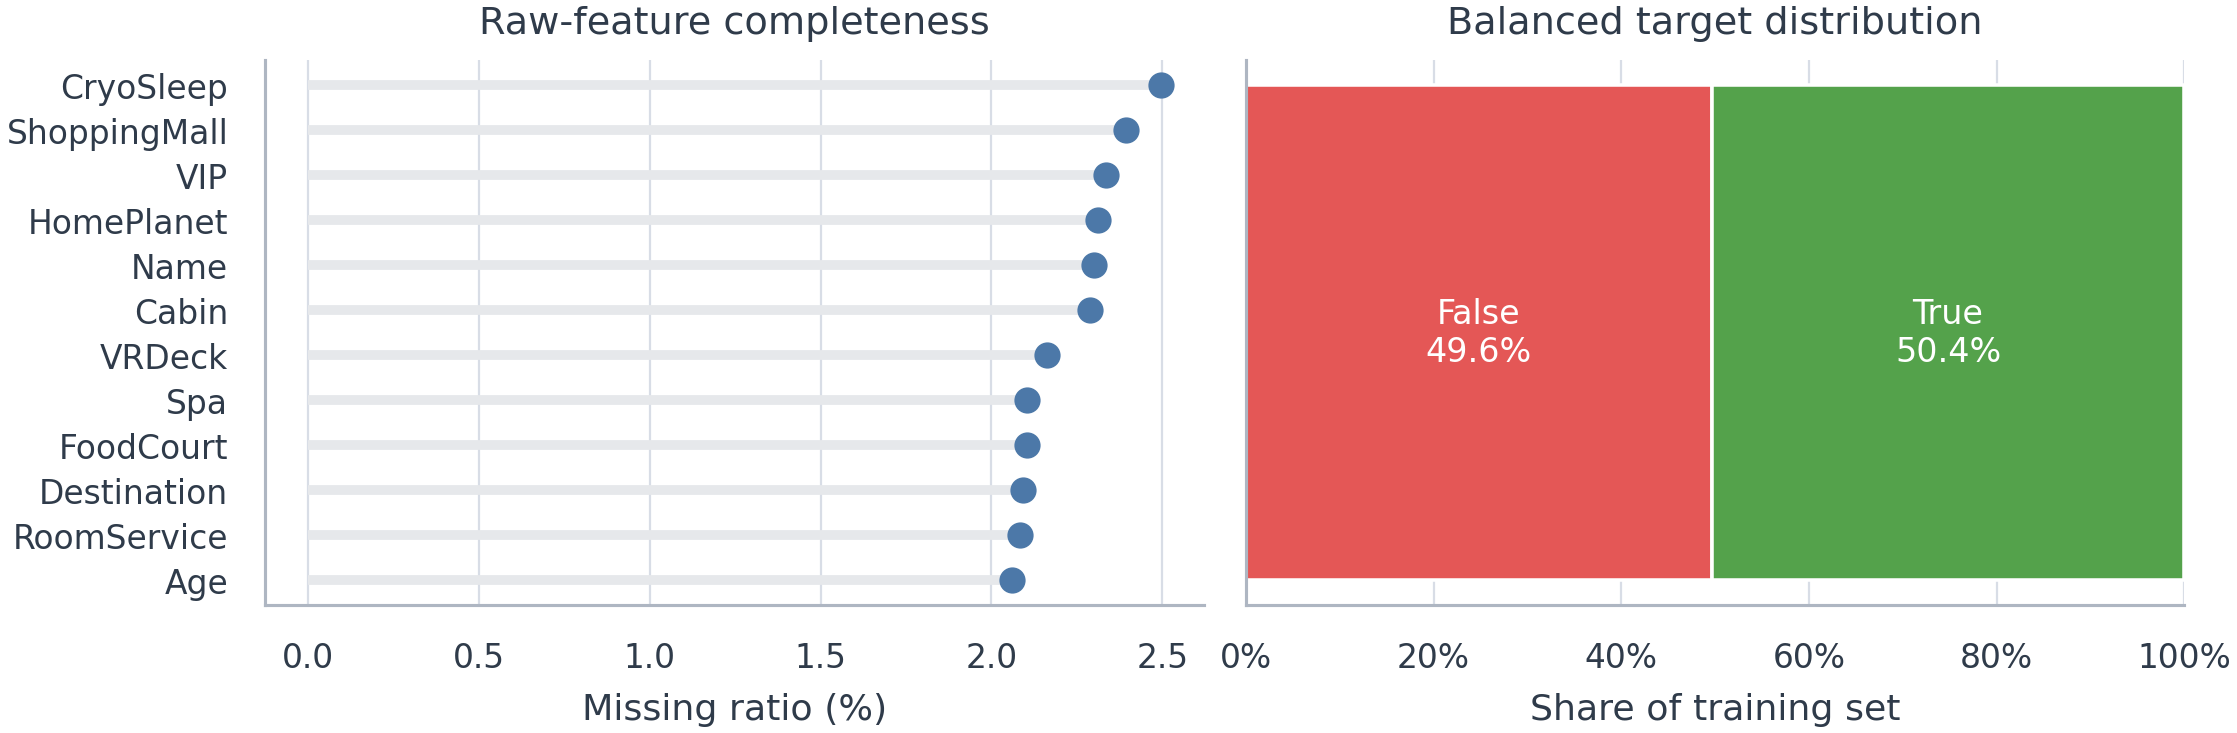
\includegraphics[width=\columnwidth]{eda_overview.png}
\caption{Data completeness and target balance. The dataset is not sparse, but careful imputation remains necessary.}
\label{fig:eda-overview}
\end{figure}

The more interesting patterns are shown in Figure~\ref{fig:eda-core}. Age contributes signal in a nonlinear way, especially when separating children from adults. Spending is much more discriminative: transported passengers are far more concentrated near zero ancillary spend, which is consistent with the domain interpretation of cryosleep. The categorical views show large rate differences across home planets and cabin decks, which motivates both category-aware models and deck-based engineered features.

\begin{figure*}[!t]
\centering
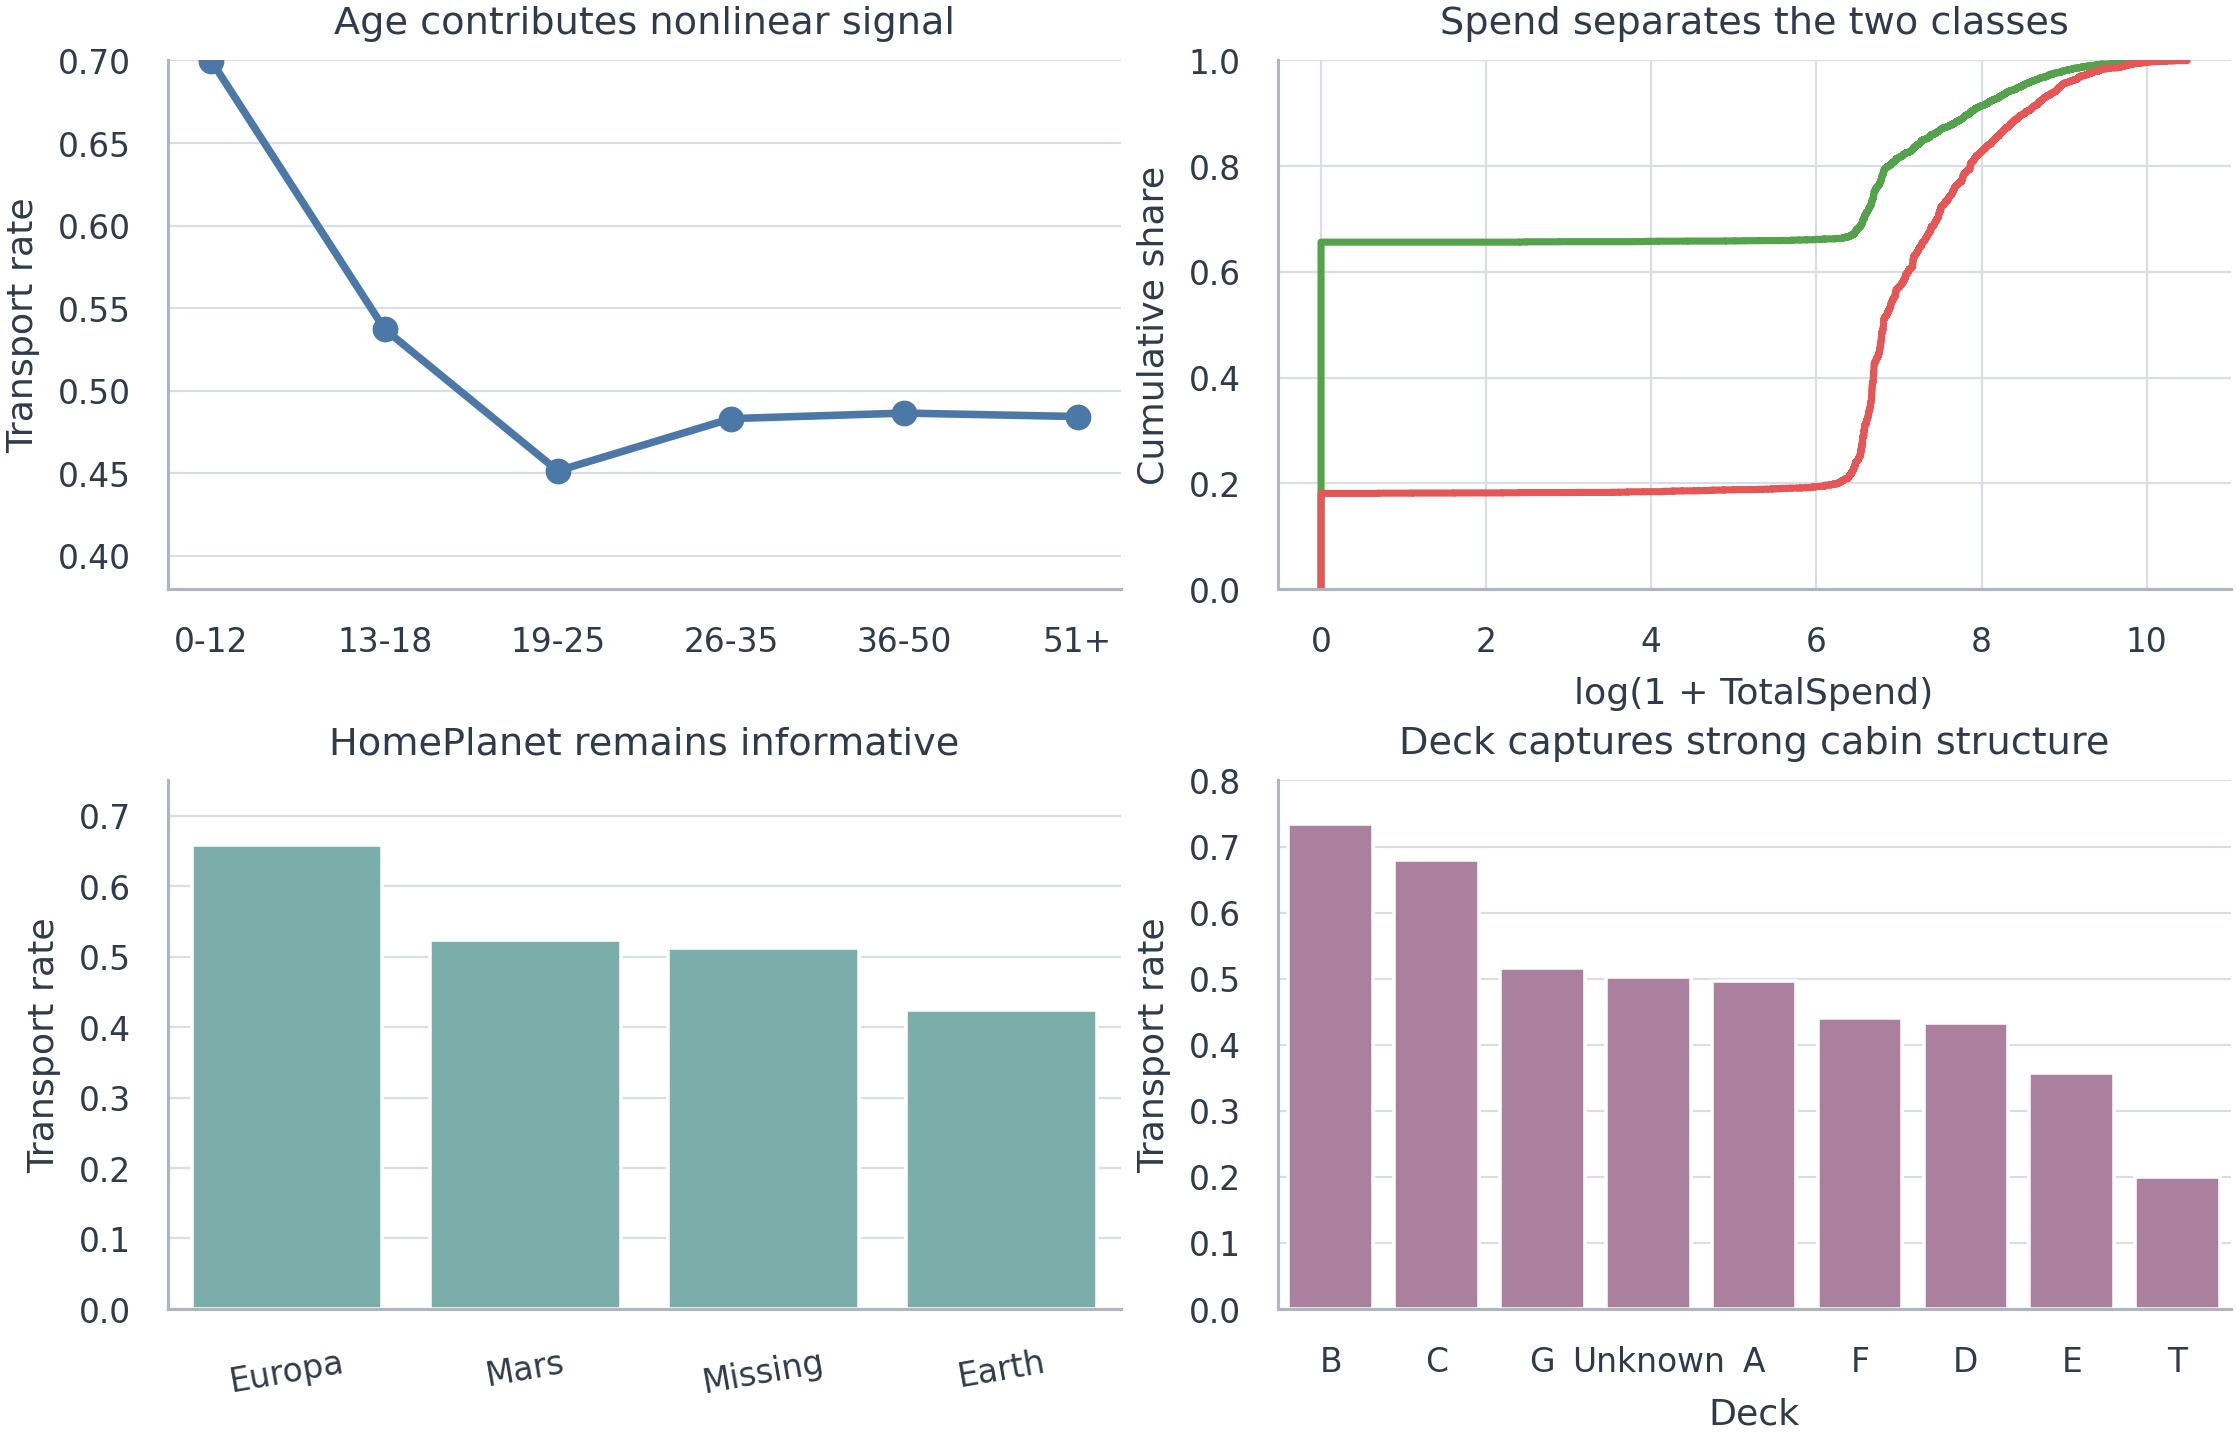
\includegraphics[width=0.96\textwidth]{eda_core_patterns.png}
\caption{Core EDA findings. Spending, home planet, and deck have clear predictive value, while age contributes weaker but still meaningful nonlinear structure.}
\label{fig:eda-core}
\end{figure*}

Figure~\ref{fig:eda-group} adds two more design cues. First, solo travelers are the single largest segment, but multi-passenger groups still occupy a large fraction of the dataset; this supports group-aware validation and explicit group features. Second, the spend variables are correlated with total spend but not perfectly redundant, which argues for keeping both aggregate and component-level information.

\begin{figure}[!t]
\centering
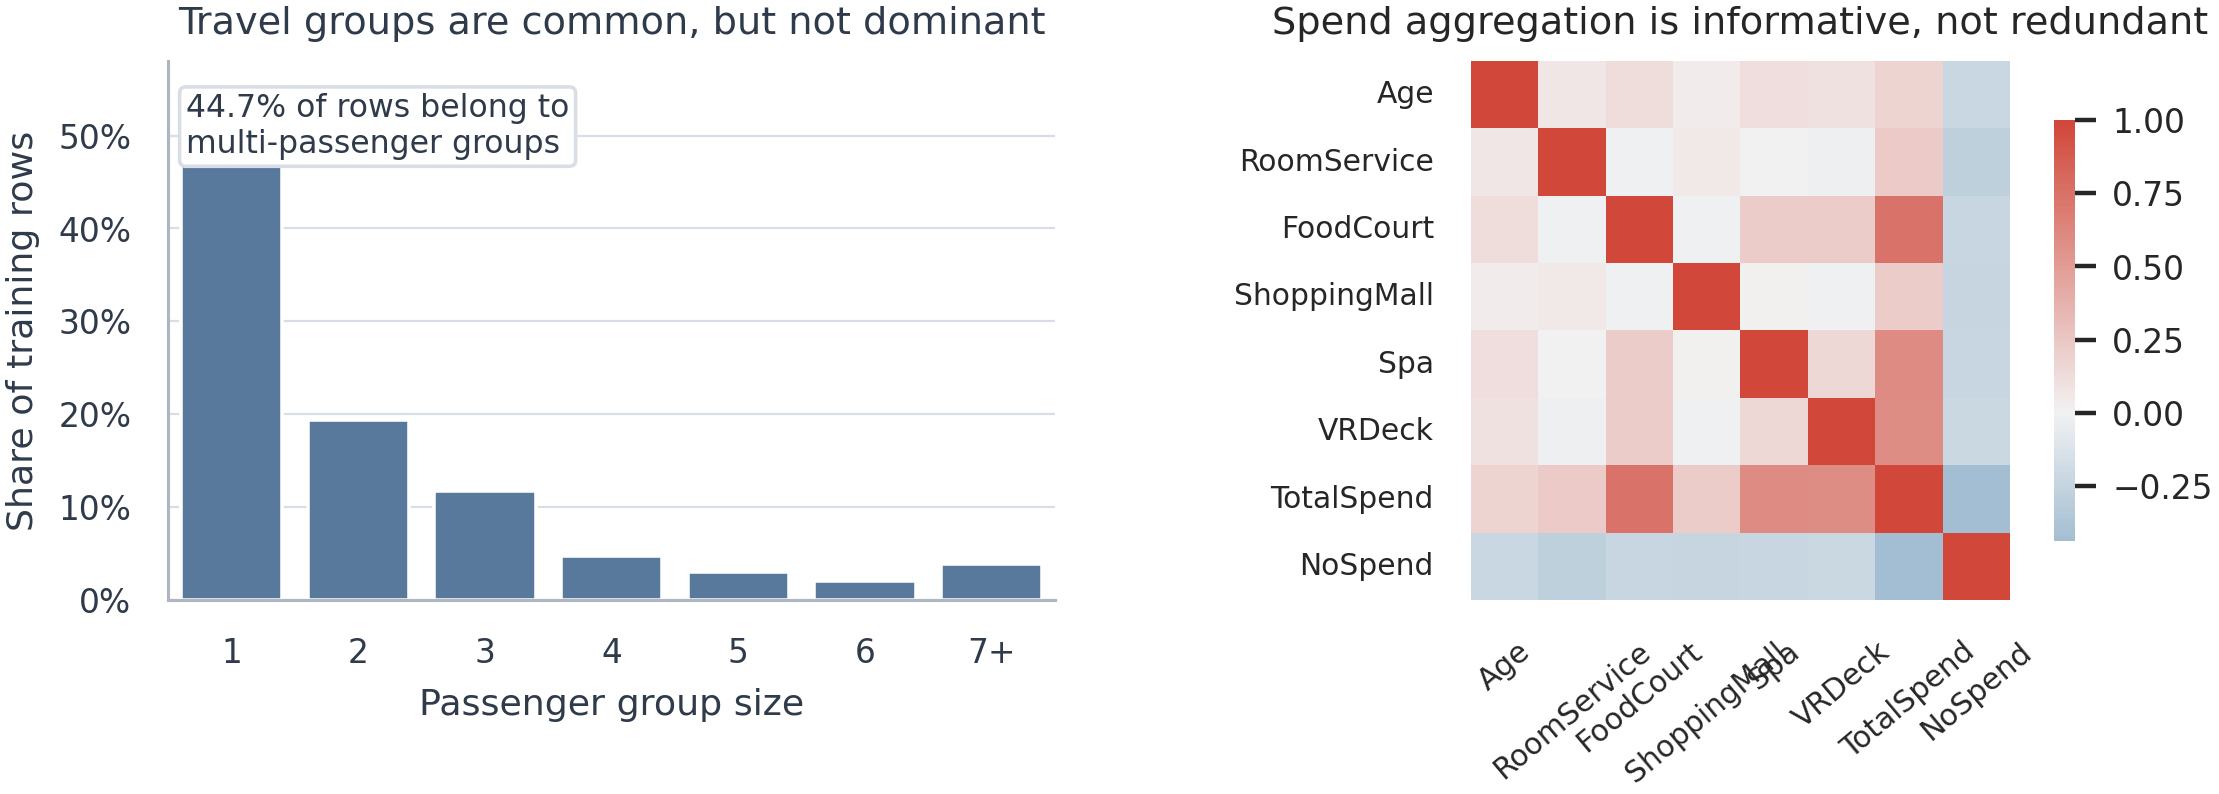
\includegraphics[width=\columnwidth]{eda_group_and_correlation.png}
\caption{Passenger-group structure and numeric correlation. These patterns motivate group-aware validation and spend aggregation instead of raw-column-only modeling.}
\label{fig:eda-group}
\end{figure}

\section{Methodology}
\subsection{Preprocessing and Feature Engineering}
Our main preprocessing rule is simple: every engineered feature must be reproducible from the official competition files alone and easy to defend during presentation. The final feature space consists of five families:
\begin{enumerate}
\item Original demographics and travel descriptors: \texttt{HomePlanet}, \texttt{Destination}, \texttt{Age}, \texttt{VIP}, and \texttt{CryoSleep}.
\item Cabin-derived features: \texttt{Deck}, \texttt{CabinNum}, \texttt{Side}, and deck-side combinations.
\item Passenger-group-derived features: \texttt{PassengerGroup}, \texttt{PassengerNo}, \texttt{GroupSize}, and \texttt{IsAlone}.
\item Spend-derived features: \texttt{TotalSpend}, zero-spend flags, spend-composition ratios, and log-transformed spend.
\item Rule-consistency features: especially cryosleep-spend consistency indicators.
\end{enumerate}

Table~\ref{tab:feature-families} summarizes these families and the intuition behind them.

\begin{table}[!t]
\caption{Engineered feature families}
\label{tab:feature-families}
\centering
\scriptsize
\begin{tabularx}{\columnwidth}{>{\raggedright\arraybackslash}p{0.28\columnwidth}X}
\toprule
Family & Rationale and examples \\
\midrule
Original demographics & \texttt{HomePlanet}, \texttt{Destination}, \texttt{Age}, \texttt{VIP}, \texttt{CryoSleep}. These preserve the official schema. \\
Cabin-derived & \texttt{Deck}, \texttt{CabinNum}, \texttt{Side}, and \texttt{DeckSide}. These encode spatial structure inside the ship. \\
Passenger-group-derived & \texttt{PassengerGroup}, \texttt{PassengerNo}, \texttt{GroupSize}, and \texttt{IsAlone}. These model travel-group behavior explicitly. \\
Spend-derived & \texttt{TotalSpend}, \texttt{NoSpend}, spend ratios, and \texttt{LogTotalSpend}. These summarize luxury-service behavior more cleanly. \\
Rule-consistency & Cryosleep-spend consistency flags. These encode plausible behavioral constraints. \\
\bottomrule
\end{tabularx}
\end{table}

\subsection{Validation Protocol}
The most important methodological choice in this project is the validation design. Because group members often share outcomes, row-level random validation leaks relational structure into the validation folds. We therefore adopted repeated \texttt{StratifiedGroupKFold} grouped by the \texttt{PassengerId} prefix.

We also separated seeds into two roles:
\begin{itemize}
\item Search seeds \texttt{\{7, 21, 42, 87, 123\}} for exploratory tuning and feature experiments.
\item Audit seeds \texttt{\{3, 11, 17, 29, 57, 68, 99, 131\}} for promotion decisions only.
\end{itemize}

Our promotion rule was conservative: a candidate should improve out-of-fold accuracy by at least 0.001 on both seed sets, while keeping the audit threshold fixed at 0.5. This rule prevented us from promoting many attractive but unstable changes.

\subsection{Model Families and Tuning Strategy}
The course requires at least four models, so we benchmarked five: Logistic Regression, Random Forest, LightGBM, XGBoost, and CatBoost. Logistic Regression and Random Forest serve as linear and bagging baselines. LightGBM, XGBoost, and CatBoost represent the dominant boosting family for tabular competitions.

Tuning strategy depended on the role of each model. The validation-first benchmark used a common feature space and repeated group-aware validation so that models remained comparable. LightGBM and CatBoost were tuned locally around strong baselines. XGBoost appeared in two different roles:
\begin{enumerate}
\item as part of the clean unified benchmark;
\item as a separate competition-side branch designed to maximize public leaderboard performance.
\end{enumerate}

The competition-side XGBoost branch intentionally relaxes some of the cleanliness constraints of the main benchmark. It concatenates train and test during categorical harmonization, performs room-guided imputation, reduces the encoded feature space from 27 to 15 dimensions through manual pruning, and finally trains a regularized XGBoost model with \texttt{max\_depth}=5, \texttt{n\_estimators}=725, \texttt{learning\_rate}=0.05, \texttt{subsample}=0.96, \texttt{colsample\_bytree}=0.93, \texttt{reg\_alpha}=4.582, and \texttt{reg\_lambda}=3.06. We report this branch separately because it was optimized for competition performance, not because it is the cleanest scientific baseline.

\begin{table}[!t]
\caption{Competition-side XGBoost branch configuration}
\label{tab:xgb-config}
\centering
\scriptsize
\begin{tabularx}{\columnwidth}{>{\raggedright\arraybackslash}p{0.36\columnwidth}X}
\toprule
Component & Setting \\
\midrule
Categorical harmonization & Train and test concatenated before categorical imputation and one-hot alignment \\
Imputation logic & Mean imputation for numeric columns, most-frequent imputation for compact categorical set, plus room-guided filling for \texttt{VIP}, \texttt{Cabin}, \texttt{HomePlanet}, and \texttt{Destination} \\
Compact branch features & 27 encoded features before pruning; 15 after pruning \\
Outlier filtering & \texttt{IsolationForest} with contamination $=0.003$; 8,666 rows retained \\
Class balancing & \texttt{KMeansSMOTE}; training rows increased to 8,761 \\
Final XGBoost setting & \texttt{max\_depth}=5, \texttt{n\_estimators}=725, \texttt{learning\_rate}=0.05, \texttt{subsample}=0.96, \texttt{colsample\_bytree}=0.93, \texttt{reg\_alpha}=4.582, \texttt{reg\_lambda}=3.06 \\
\bottomrule
\end{tabularx}
\end{table}

\subsection{Experimental Controls and Reproducibility}
To keep the report defensible, we maintained several controls across the validation-first benchmark. All unified model comparisons used the same feature families, the same group-aware split design, the same fixed threshold on audit seeds, and no external prediction files. This makes the benchmark table interpretable as a true model-family comparison rather than a comparison between unrelated pipelines.

We also maintained separate tuning evidence for the clean benchmark models. In the copied workspace logs, the LightGBM random-search winner improved audit accuracy by +0.0031 over the default baseline, while the best CatBoost sweep improved audit accuracy by +0.0023. We report these gains explicitly later because the course brief requires hyperparameter tuning to be demonstrated rather than merely asserted.

We deliberately isolated the competition-side XGBoost branch from this benchmark. Its purpose was different: maximize public leaderboard score within the official competition rules. By separating the two tracks, we avoided a common failure mode in course reports where a leaderboard-oriented branch silently becomes the ``best model'' even when it is no longer the cleanest scientific baseline.

\section{Experimental Study and Results}
\subsection{Unified Local Benchmark}
Table~\ref{tab:benchmark} reports mean CV accuracy, OOF F1, OOF AUC, training time, inference cost, and artifact size under the same benchmark scaffold. This satisfies the course requirement that models be compared by both performance and practicality.

\begin{table*}[!t]
\caption{Unified local benchmark under the same feature set and validation regime}
\label{tab:benchmark}
\centering
\scriptsize
\begin{tabular}{lcccccc}
\toprule
Model & Mean CV Acc. & OOF F1 & OOF AUC & CV Fit Time (s) & Test Infer. (ms/sample) & Artifact Size (MB) \\
\midrule
CatBoost & 0.8135 & 0.8143 & 0.9069 & 288.32 & 0.0230 & 1.37 \\
XGBoost & 0.8106 & 0.8103 & 0.9034 & 3.19 & 0.0061 & 1.04 \\
LightGBM & 0.8086 & 0.8099 & 0.9012 & 5.20 & 0.0089 & 1.65 \\
Random Forest & 0.8062 & 0.8013 & 0.8930 & 4.79 & 0.0350 & 62.40 \\
Logistic Regression & 0.7987 & 0.8047 & 0.8887 & 0.46 & 0.0040 & 0.01 \\
\bottomrule
\end{tabular}
\end{table*}

The ranking is visually summarized in Figure~\ref{fig:benchmark}. CatBoost is the strongest local model, XGBoost is only slightly weaker while being dramatically faster to train, and the linear baseline underfits the task.

\begin{figure}[!t]
\centering
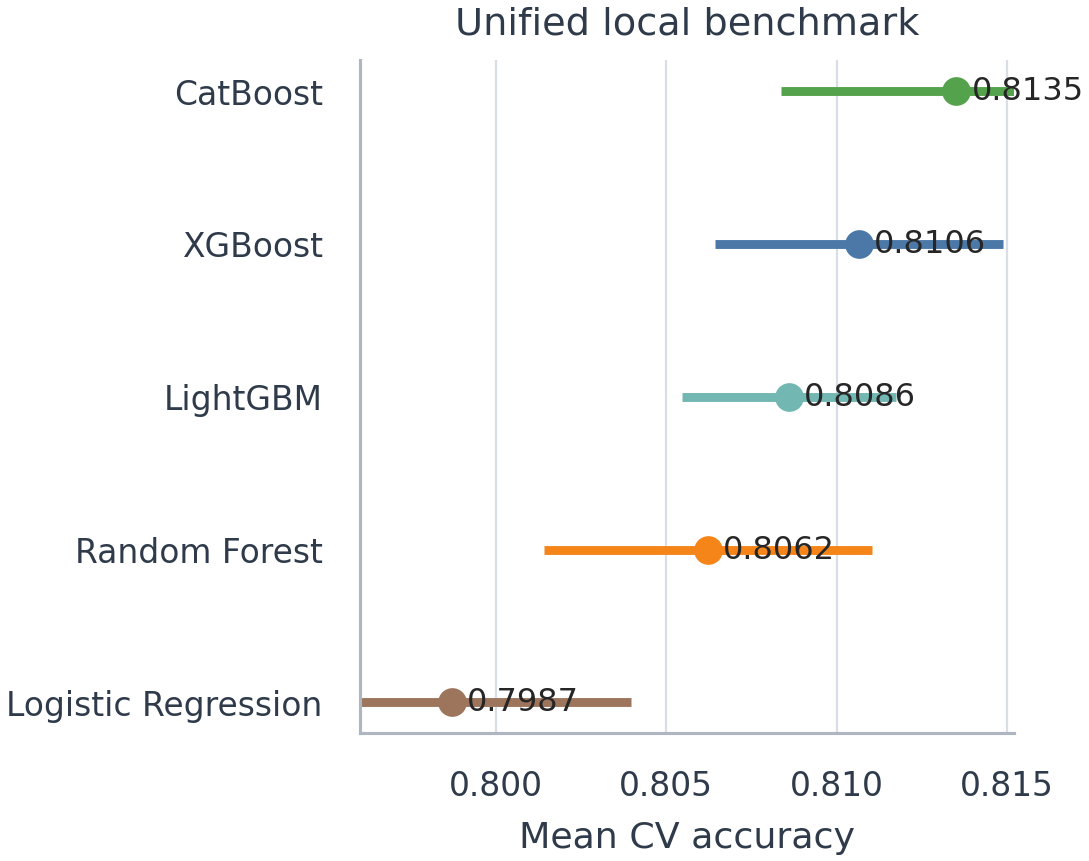
\includegraphics[width=\columnwidth]{model_benchmark.png}
\caption{Mean CV accuracy under the unified benchmark. Boosting clearly dominates the task.}
\label{fig:benchmark}
\end{figure}

\begin{figure}[!t]
\centering
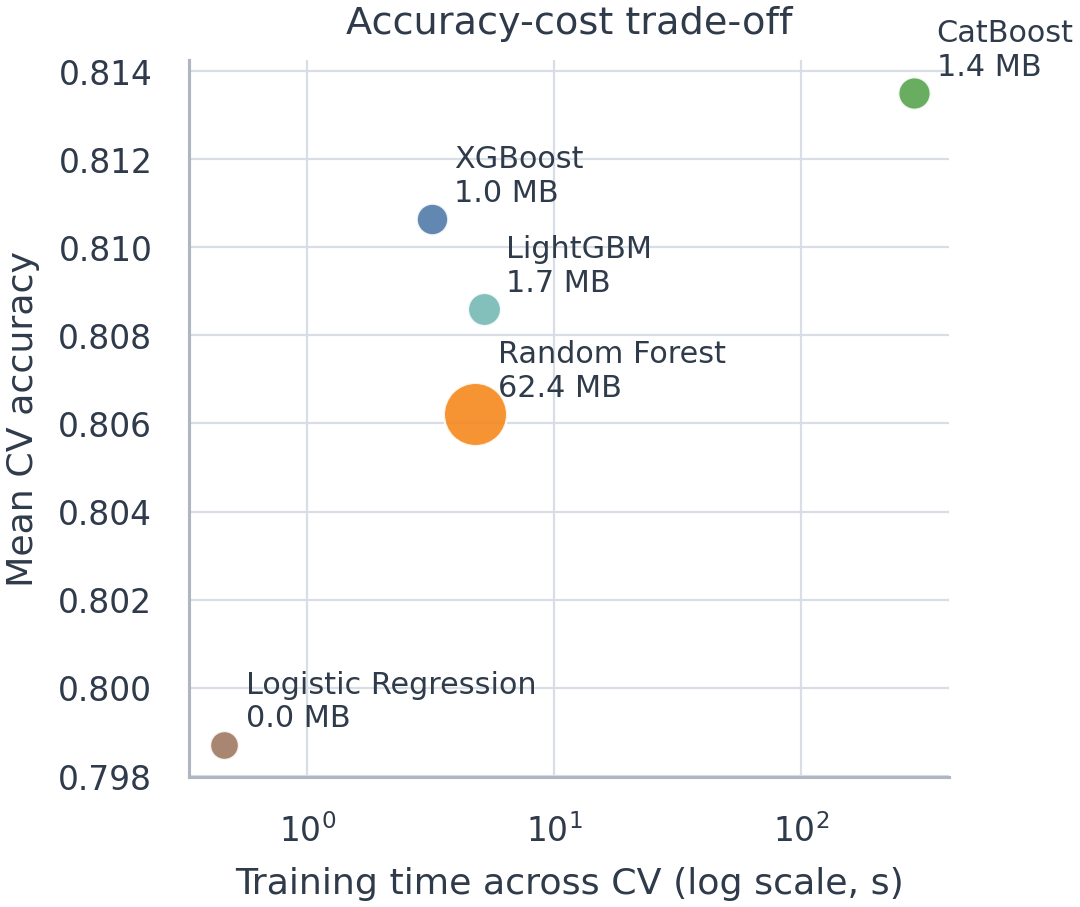
\includegraphics[width=\columnwidth]{model_efficiency_tradeoff.png}
\caption{Accuracy-cost trade-off. CatBoost is strongest locally, while XGBoost is the most attractive speed-performance compromise.}
\label{fig:efficiency}
\end{figure}

\subsection{Why the Models Behave Differently}
The benchmark is informative not only for ranking models, but also for explaining fit to the data. Logistic Regression is weakest because the task contains interacting nonlinear effects: cryosleep interacts with spending, passenger groups interact with cabin information, and cabin identifiers only become informative after decomposition. Random Forest improves on the linear baseline by modeling interactions, but it pays a large memory cost without matching the boosted methods.

LightGBM and XGBoost fit the task more naturally. Both exploit nonlinear interactions and support fast iteration on encoded tabular features. CatBoost performs best locally because the dataset contains exactly the kind of mixed categorical and numerical structure for which CatBoost is especially strong. This aligns with our EDA findings: home planet, deck, side, group, and spending all interact in ways richer than a purely numeric benchmark, but still well within the regime where classical boosted trees excel.

Table~\ref{tab:model-suitability} summarizes these qualitative fit arguments.

\begin{table*}[!t]
\caption{Qualitative suitability of each benchmarked model for this dataset}
\label{tab:model-suitability}
\centering
\scriptsize
\begin{tabularx}{\textwidth}{>{\raggedright\arraybackslash}p{0.14\textwidth}X X X}
\toprule
Model & Main strengths on this task & Main weaknesses on this task & Overall suitability \\
\midrule
Logistic Regression & Very fast, interpretable, and useful as a sanity-check baseline. & Cannot capture nonlinear cryosleep-spend-group interactions compactly. & Low. Good baseline, weak final model. \\
Random Forest & Flexible nonlinear baseline with few distributional assumptions. & Large artifact size and weaker score than boosting under the same feature space. & Moderate. Reasonable baseline, not the best trade-off here. \\
LightGBM & Fast training and strong performance on sparse encoded features. & Small local gains proved unstable under wider audit checks. & High. Strong clean benchmark model. \\
XGBoost & Best speed-performance compromise and highly competitive competition model. & Sensitive to preprocessing and feature-pruning choices. & High. Strong practical model, especially for the competition-side branch. \\
CatBoost & Best local accuracy and very natural fit for mixed-type tabular data. & Slower to train; not the top public-score branch. & Very high. Best scientific anchor for the final report. \\
\bottomrule
\end{tabularx}
\end{table*}

\subsection{Interpretability of the Clean CatBoost Anchor}
The clean CatBoost anchor is also the easiest model to interpret. Figure~\ref{fig:catboost-importance} shows the top feature importances extracted from the validation-first CatBoost benchmark. \texttt{TotalSpend}, \texttt{Deck}, \texttt{HomePlanet}, and \texttt{PassengerGroup} dominate the ranking, which is consistent with the strongest EDA signals. The same figure also explains why the clean CatBoost pipeline is such a good report centerpiece: the leading signals are semantically meaningful and align with domain intuition instead of depending on opaque post-processing.

\begin{figure}[!t]
\centering
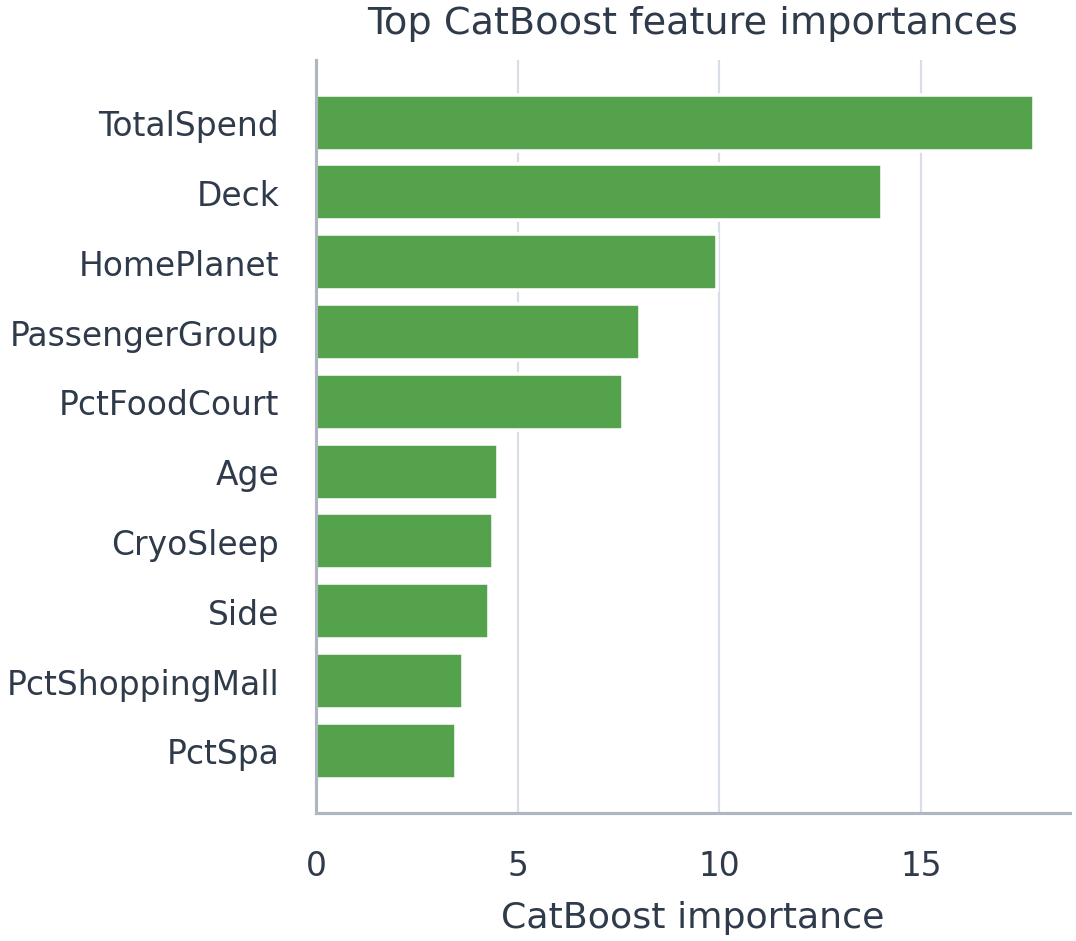
\includegraphics[width=\columnwidth]{catboost_feature_importance.png}
\caption{Top feature importances from the clean CatBoost anchor. The strongest signals align well with the EDA findings.}
\label{fig:catboost-importance}
\end{figure}

\subsection{Feature-Family Ablation}
To test whether every plausible feature family was actually helpful, we ran a cumulative ablation study on the clean CatBoost line under the same group-aware validation protocol. Figure~\ref{fig:feature-ablation} summarizes the result.

\begin{figure}[!t]
\centering
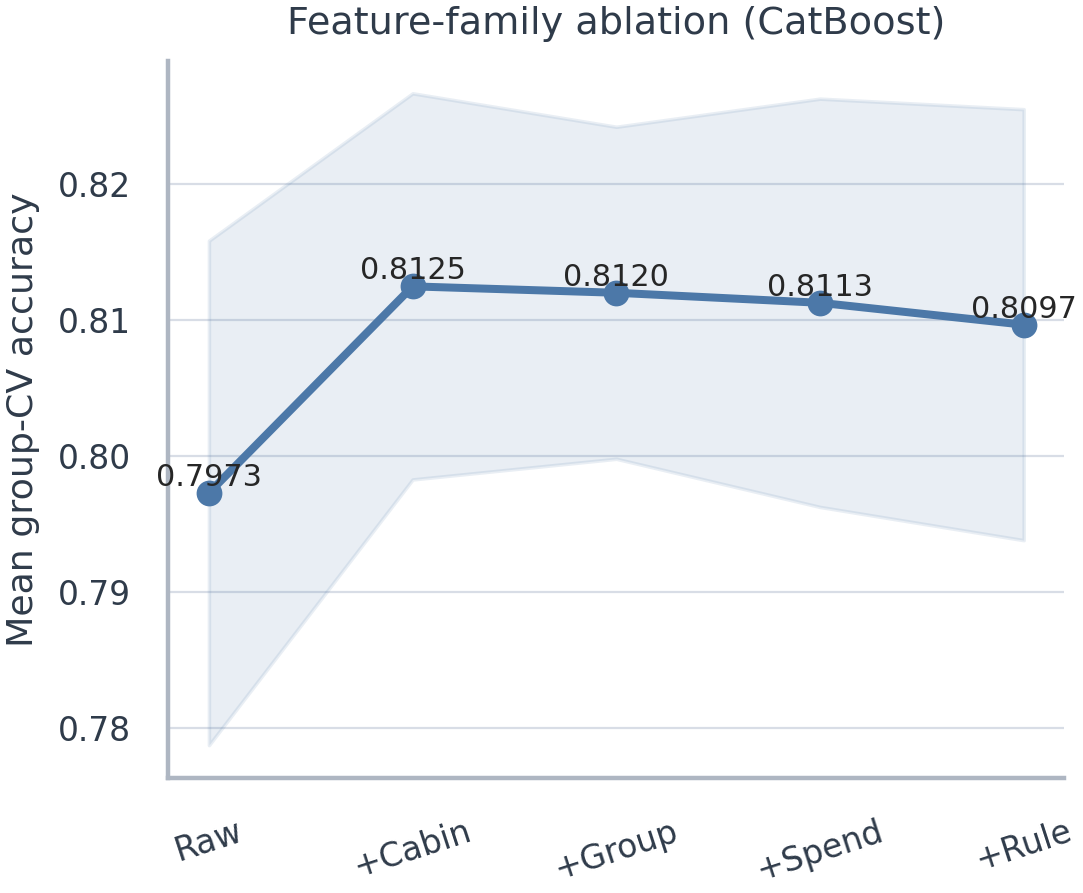
\includegraphics[width=\columnwidth]{feature_ablation.png}
\caption{Cumulative feature-family ablation on the clean CatBoost line. Cabin decomposition produced the largest single improvement.}
\label{fig:feature-ablation}
\end{figure}

The pattern is more informative than a simple ``more features is better'' narrative. Raw official features alone reached only 0.7973. Adding cabin decomposition raised group-aware CV to 0.8125, which was the largest jump in the entire study. Adding group features kept performance near the same level, while spend-summary and rule-consistency features provided no further gain under this fixed CatBoost setting and slightly reduced the final mean. This does not mean that group or spend information is useless. Rather, under this particular CatBoost configuration, those later families are partly redundant with the already strong cabin-enhanced core representation instead of being additively beneficial. That finding supports our conservative promotion rule and shows that the final report is not based on blind feature accumulation.

\subsection{Tuning Evidence on Clean Models}
Figure~\ref{fig:tuning-summary} summarizes the audited gains from the two clean-model tuning tracks that were preserved in the workspace notes.

\begin{figure}[!t]
\centering
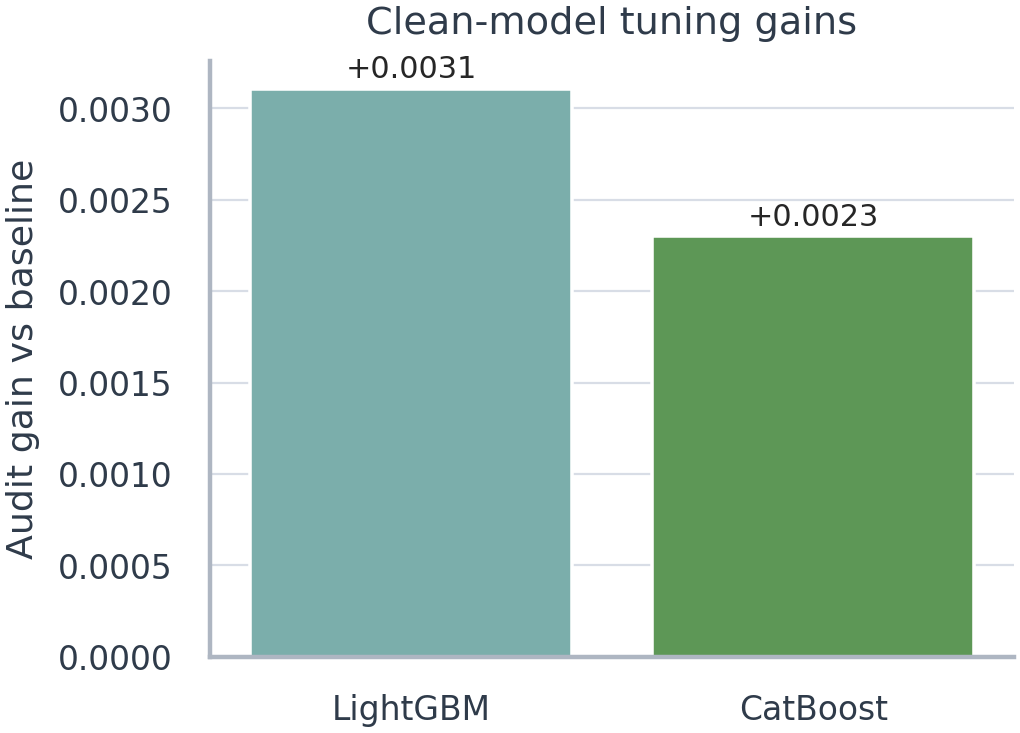
\includegraphics[width=\columnwidth]{tuning_summary.png}
\caption{Audited tuning gains for the clean LightGBM and CatBoost search tracks preserved in the local experiment logs.}
\label{fig:tuning-summary}
\end{figure}

The LightGBM search track improved audit accuracy by +0.0031 over its default baseline through random search with independent audit seeds. The CatBoost sweep improved audit accuracy by +0.0023 over the clean baseline through a smaller local parameter sweep. These deltas are meaningful enough to satisfy the course requirement for hyperparameter tuning, while still remaining inside a report-standard workflow.

Table~\ref{tab:tuning-key-changes} makes the tuning path more concrete. The winning LightGBM candidate became smaller in leaf capacity, deeper in explicit tree depth, and more conservative through stronger regularization and larger minimum leaf size. The winning CatBoost candidate moved in a similar direction: slightly deeper trees, stronger $L_2$ regularization, modest subsampling, and less aggressive feature sampling noise. In other words, the preserved search evidence points to disciplined regularization and capacity control rather than to exotic hyperparameter tricks.

\begin{table*}[!t]
\caption{Key hyperparameter changes preserved in the clean tuning logs}
\label{tab:tuning-key-changes}
\centering
\scriptsize
\begin{tabularx}{\textwidth}{>{\raggedright\arraybackslash}p{0.12\textwidth}X X c}
\toprule
Model & Baseline setting & Tuned winner setting & Audit gain \\
\midrule
LightGBM & 500 trees, 31 leaves, unlimited depth, \texttt{subsample}=0.90, \texttt{colsample}=0.80, \texttt{reg\_alpha}=0.10, \texttt{min\_child\_samples}=25 & 1000 trees, 15 leaves, depth 6, full row/column sampling, \texttt{reg\_alpha}=0.70, \texttt{min\_child\_samples}=35 & +0.0031 \\
CatBoost & depth 6, \texttt{l2\_leaf\_reg}=3, \texttt{subsample}=0.80, \texttt{rsm}=1.00, \texttt{random\_strength}=1, \texttt{min\_data\_in\_leaf}=1 & depth 7, \texttt{l2\_leaf\_reg}=7, \texttt{subsample}=0.88, \texttt{rsm}=0.85, \texttt{random\_strength}=0.5, \texttt{min\_data\_in\_leaf}=8 & +0.0023 \\
\bottomrule
\end{tabularx}
\end{table*}

\subsection{Validation Alignment versus Public Leaderboard}
One of the central findings of the project is that local validation and public leaderboard behavior do not align monotonically. Figure~\ref{fig:cv-public} shows this directly. The most striking counterexample is the clean \texttt{Opamusora} CatBoost candidate, which reached 0.81905 under local group-aware validation but only 0.80593 publicly. The inverse pattern is the team's public-best XGBoost branch, which achieved only 0.80516 under our strict group-aware audit but scored 0.81716 on the public leaderboard.

\begin{figure}[!t]
\centering
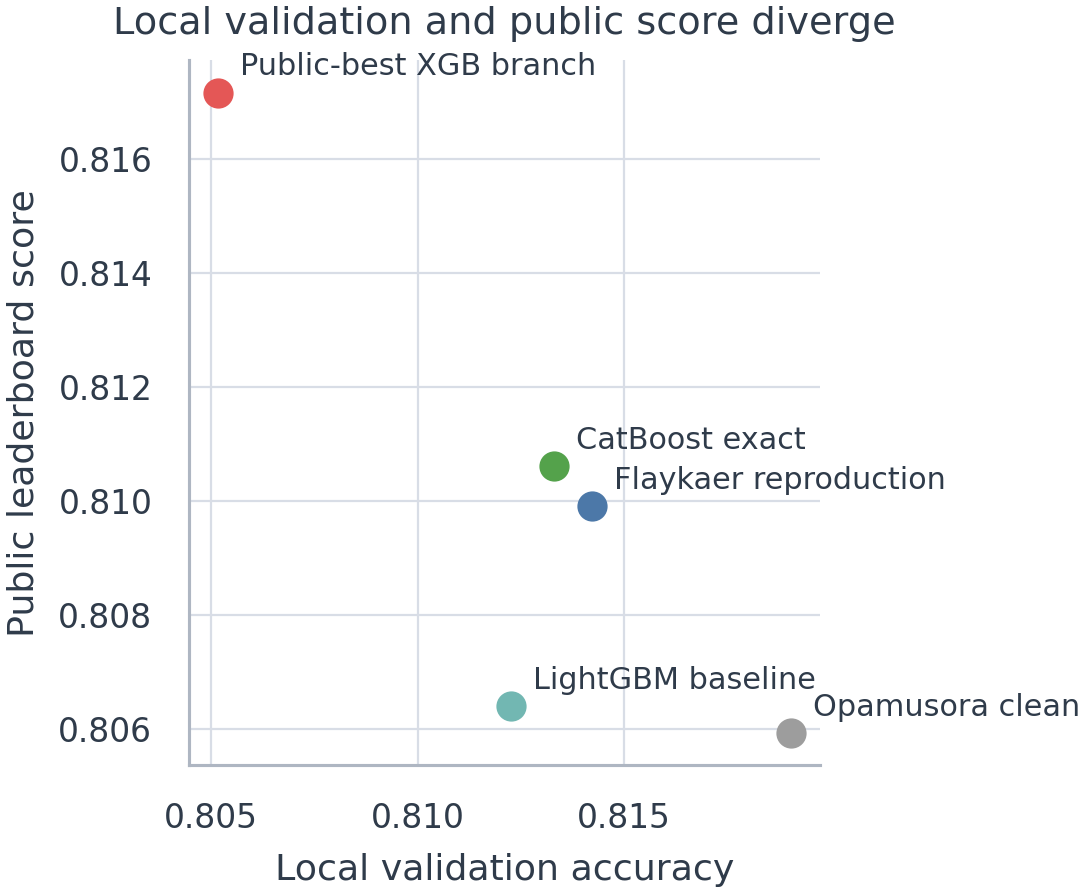
\includegraphics[width=\columnwidth]{cv_vs_public.png}
\caption{Local validation does not monotonically predict public leaderboard score. This is why the report emphasizes validation design and ablation rather than public-score chasing alone.}
\label{fig:cv-public}
\end{figure}

This mismatch changed our workflow. First, we stopped trusting tiny local improvements unless they survived the audit seeds. Second, we separated the best clean single model from the best public submission instead of forcing one narrative to explain both. The best clean single model in the workspace remains the CatBoost exact pipeline, which scored 0.81061 publicly and is straightforward to explain. The best public result belongs to a different XGBoost branch with a different objective.

Table~\ref{tab:representative-lines} summarizes the candidate lines that mattered most to this conclusion. The table is useful because it separates three different concepts that are easy to blur together in a Kaggle report: the strongest clean scientific anchor, the strongest local-CV counterexample, and the strongest public-leaderboard branch.

\begin{table*}[!t]
\caption{Representative candidate lines and what they taught us}
\label{tab:representative-lines}
\centering
\scriptsize
\begin{tabularx}{\textwidth}{>{\raggedright\arraybackslash}p{0.19\textwidth}cc>{\raggedright\arraybackslash}p{0.18\textwidth}X}
\toprule
Candidate line & Local metric & Public score & Role in the project & Main lesson \\
\midrule
LightGBM baseline & 0.81226 & 0.80640 & Early validation-first baseline & Useful baseline for promotion decisions, but not strong enough as a final competition submission. \\
CatBoost exact & 0.81330 & 0.81061 & Best clean single-model anchor & The most defensible report centerpiece: strong score, simple preprocessing, and high interpretability. \\
Flaykaer reproduction & 0.81422 & 0.80991 & Transparent clean reproduction & Good example of a respectable public reproduction that still failed to beat the clean anchor. \\
Opamusora clean & 0.81905 & 0.80593 & High-CV counterexample & Strongest evidence that local group-aware CV alone is not a dependable public-score ranker near the top of this competition. \\
Public-best XGB branch & 0.80516 & 0.81716 & Best leaderboard branch & Highest public result, but not the strongest scientific baseline; must be explained as a separate competition-side line. \\
\bottomrule
\end{tabularx}
\end{table*}

\subsection{The XGBoost Exploration Branch}
The highest public score in the team history did not appear from a single isolated submission. It emerged through an XGBoost-centered exploration line. Figure~\ref{fig:xgb-branch} shows this trajectory. An early single XGBoost submission reached 0.79378 on April 1, 2026, a revised single-model version reached 0.80383 on April 10, 2026, XGBoost-assisted stacking reached 0.81084 on April 16, 2026, and the final public-best XGBoost branch reached 0.81716 on April 26, 2026.

This distinction is important because we do not claim that the final XGBoost parameters are a magical local-CV optimum. Instead, we claim something narrower and more reproducible: the public-best branch is backed by a visible experimental provenance. The parameter set came from the Optuna-labeled compact XGBoost notebook that seeded this branch; the pipeline was then reconstructed as a standalone training path; a small Optuna rerun in the cleaned demo repository confirmed that nearby regularized XGBoost settings are plausible under the same compact feature space; and a focused neighborhood search showed that the final parameters lie inside a competitive plateau rather than far away from reasonable alternatives. Thus, the public-best submission should be read as an evidence-backed competition artifact, not as a parameter choice made by guesswork.

\begin{figure*}[!t]
\centering
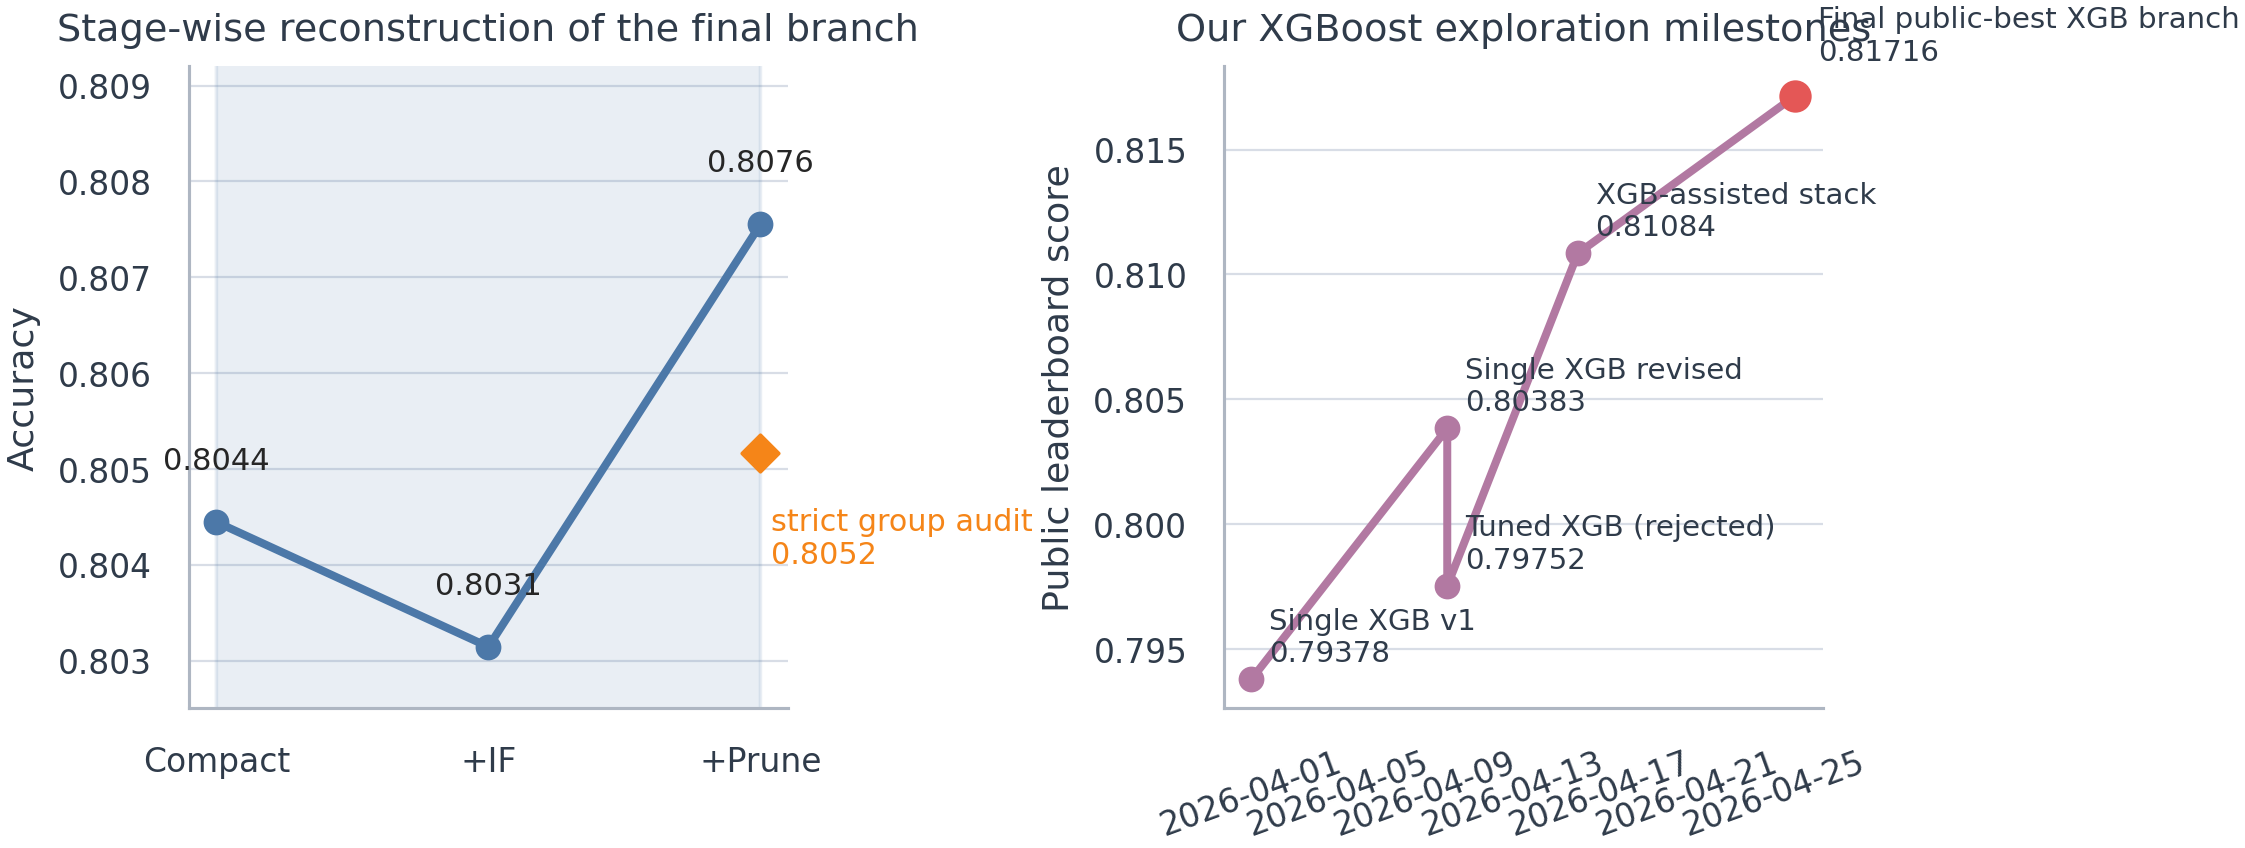
\includegraphics[width=0.96\textwidth]{xgb_branch_evolution.png}
\caption{Left: stage-wise reconstruction of the final XGBoost branch. Right: the public-score trajectory of our XGBoost-centered exploration path from April 1, 2026 to April 26, 2026.}
\label{fig:xgb-branch}
\end{figure*}

To understand why the final branch worked, we reconstructed it in stages and measured how its local behavior changed. Table~\ref{tab:xgb-stage} reports the result. The compact preprocessing branch itself only reached 0.80445 under 10-fold row-level reconstruction CV. IsolationForest filtering actually made this reconstruction metric worse, while feature pruning raised it to 0.80755. Re-evaluated under our stricter 5-fold \texttt{StratifiedGroupKFold} audit, the same branch scored 0.80516.

\begin{table*}[!t]
\caption{Stage-wise reconstruction of the final XGBoost branch}
\label{tab:xgb-stage}
\centering
\scriptsize
\begin{tabularx}{\textwidth}{>{\raggedright\arraybackslash}p{0.28\textwidth}>{\raggedright\arraybackslash}p{0.22\textwidth}ccX}
\toprule
Stage & Validation view & Accuracy & Std. dev. & Interpretation \\
\midrule
Compact preprocessing branch & 10-fold row-level reconstruction CV & 0.80445 & 0.01417 & A workable but not yet competitive compact XGBoost baseline. \\
+ IsolationForest filtering & 10-fold row-level reconstruction CV & 0.80314 & 0.01590 & Outlier filtering did not help locally and would not have been promoted on a scientific track. \\
+ Feature pruning & 10-fold row-level reconstruction CV & 0.80755 & 0.01542 & Manual pruning recovered a clearer gain and created the final compact branch used for the public-best submission. \\
Strict group-aware audit & 5-fold StratifiedGroupKFold & 0.80516 & 0.00490 & Under the stricter report-standard audit, the branch remains weaker than the clean CatBoost anchor despite its public success. \\
\bottomrule
\end{tabularx}
\end{table*}

Table~\ref{tab:xgb-milestones} makes the public-side evolution explicit. The rejected tuned XGBoost variant on April 10, 2026 is especially informative: tuning alone did not help, and the real breakthrough came only after the project explored XGBoost as part of a broader competition branch rather than as a naive single-model replacement.

\begin{table*}[!t]
\caption{Milestones in the XGBoost exploration branch}
\label{tab:xgb-milestones}
\centering
\scriptsize
\begin{tabularx}{\textwidth}{>{\raggedright\arraybackslash}p{0.12\textwidth}>{\raggedright\arraybackslash}p{0.19\textwidth}cX}
\toprule
Date & Milestone & Public score & Why it mattered \\
\midrule
2026-04-01 & Single XGB v1 & 0.79378 & Established an early XGBoost baseline and showed that a straightforward single-model configuration was not yet competitive. \\
2026-04-10 & Single XGB revised & 0.80383 & Confirmed that XGBoost could improve materially with better preprocessing, even before branch-level redesign. \\
2026-04-10 & Tuned XGB (rejected) & 0.79752 & Demonstrated that naive tuning did not help and that parameter changes alone were insufficient. \\
2026-04-16 & XGB-assisted stack & 0.81084 & Showed that XGBoost became useful as a controlled component inside a stronger blended system. \\
2026-04-26 & Final public-best XGB branch & 0.81716 & Produced the highest public score in the team history and finalized the competition-side narrative. \\
\bottomrule
\end{tabularx}
\end{table*}

We also ran a focused local neighborhood search around the final branch parameters to test whether the public-best configuration was at least locally competitive under standard validation. Figure~\ref{fig:xgb-neighborhood} shows the result. Row-level CV slightly preferred a lower learning rate with more trees, while the group-aware audit slightly preferred a leaner sampling setting. However, all tested variants stayed within a narrow accuracy band, and none emerged as a dominant local winner under both views simultaneously.

\begin{figure}[!t]
\centering
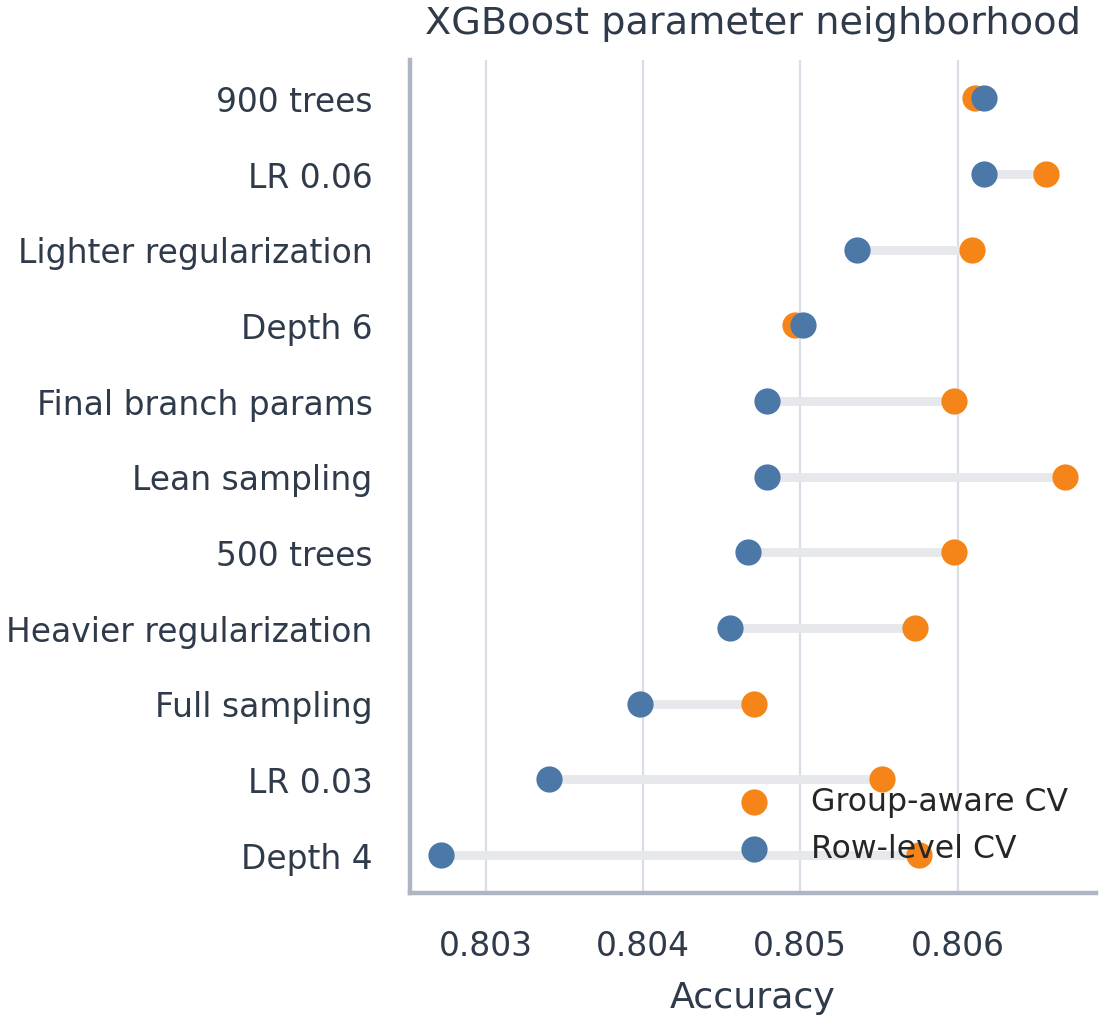
\includegraphics[width=\columnwidth]{xgb_neighborhood_search.png}
\caption{Focused local neighborhood search around the final XGBoost branch. The public-best configuration sits inside a competitive local plateau rather than as a dominant local optimum.}
\label{fig:xgb-neighborhood}
\end{figure}

This is an important result for the logic of the paper. It means the final public-best XGBoost branch should not be oversold as the unique locally optimal model. A more honest interpretation is that it lies inside a competitive parameter region, and its public superiority depends on leaderboard interaction in a way that local CV does not fully explain. That framing is much stronger academically than claiming a tuning triumph that the local evidence does not support.

Two points follow from this table. First, the final branch is not a single miraculous parameter point; it is the endpoint of a longer XGBoost exploration line in our own submission history. Second, the branch is best interpreted as a competition-side artifact rather than as our strongest scientific baseline. Its public success is real, but the strongest methodological claim of the paper still comes from the validation-first benchmark.

\subsection{Where the Two Branches Disagree}
The previous subsection explains why the public-best XGBoost branch should not be described as a universal local optimum. A complementary question is whether it at least behaves like a uniformly stronger classifier than the cleaner CatBoost line. Under one shared 5-fold \texttt{StratifiedGroupKFold} audit, the answer is no. The two branches disagree on 8.49\% of training rows, and the cleaner CatBoost line keeps a 0.37-point accuracy advantage overall under that shared audit.

Figure~\ref{fig:branch-disagreement} shows where that disagreement concentrates. At the cabin level, the two branches diverge most strongly on decks E and G. At the behavioral level, disagreement is highest in cryosleep-spend edge cases, especially passengers with missing \texttt{CryoSleep} but zero spend and passengers with \texttt{CryoSleep=False} but zero spend. These are precisely the kinds of ambiguous cases where heuristic competition-side preprocessing can change predictions substantially. Importantly, XGBoost is not uniformly worse either: it is slightly better on some narrower subsets such as Deck A and Deck E. The right interpretation is therefore a specialization story. The compact XGBoost branch changes a small but meaningful subset of decisions, some of which help publicly, but it does not dominate the cleaner CatBoost line across the board.

\begin{figure*}[!t]
\centering
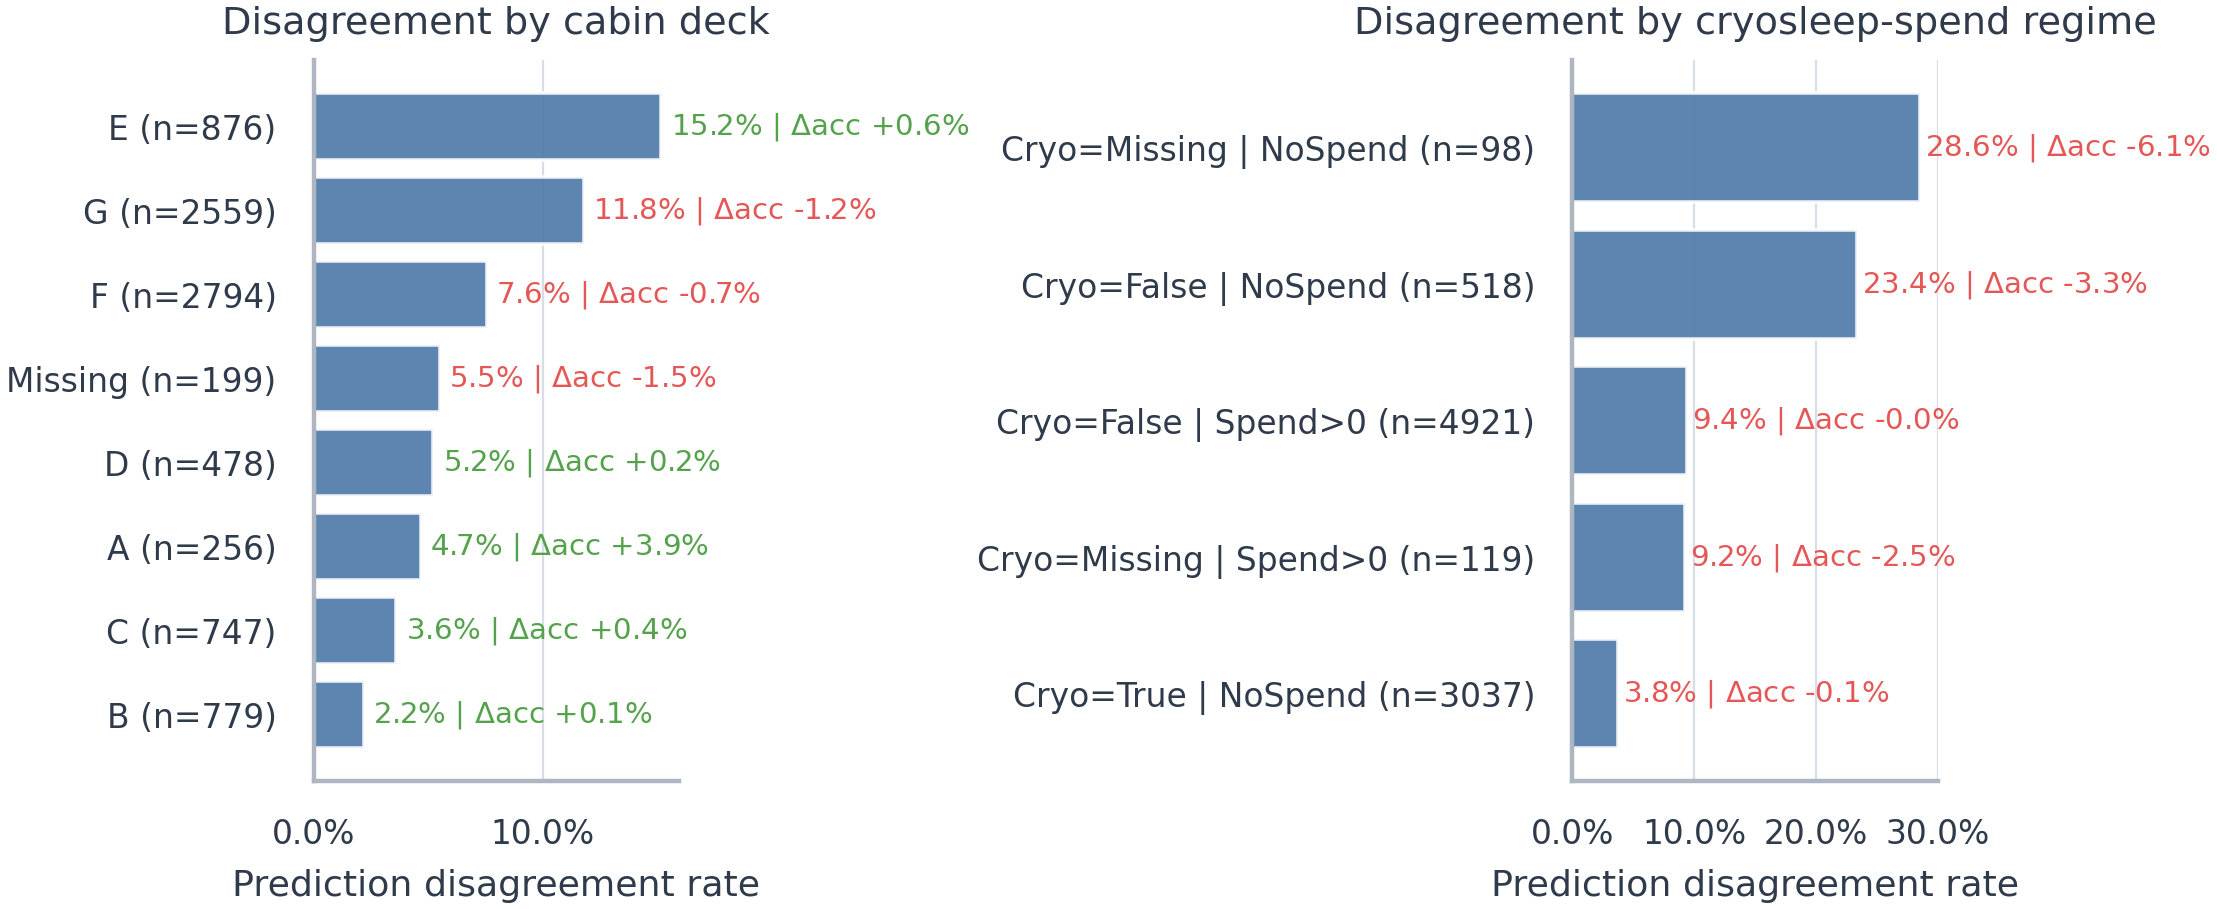
\includegraphics[width=0.96\textwidth]{branch_disagreement.png}
\caption{Shared-audit disagreement between the clean CatBoost line and the compact XGBoost branch. Text annotations report subgroup disagreement rate and local accuracy gap (XGBoost minus CatBoost).}
\label{fig:branch-disagreement}
\end{figure*}

\subsection{Final Kaggle Ranking and Submission History}
The public leaderboard snapshot downloaded on May 17, 2026 places our team \texttt{EAP\_Hater@MLW} at Rank 97 out of 2240 teams with a score of 0.81716. This corresponds to approximately the top 4.3\% of ranked teams in the downloaded snapshot. The best clean single-model submission reached 0.81061 and Rank 238.

Figure~\ref{fig:timeline} shows the overall public-score trajectory, while Figure~\ref{fig:leaderboard} situates our score inside the distribution of all public leaderboard scores. For course-compliance purposes, Figure~\ref{fig:submissionlog} also includes a curated snapshot of representative Kaggle submission milestones retrieved through the Kaggle API on May 17, 2026. Semantic labels are used for readability, while the raw submission history is preserved in the exported tables.

\begin{figure}[!t]
\centering
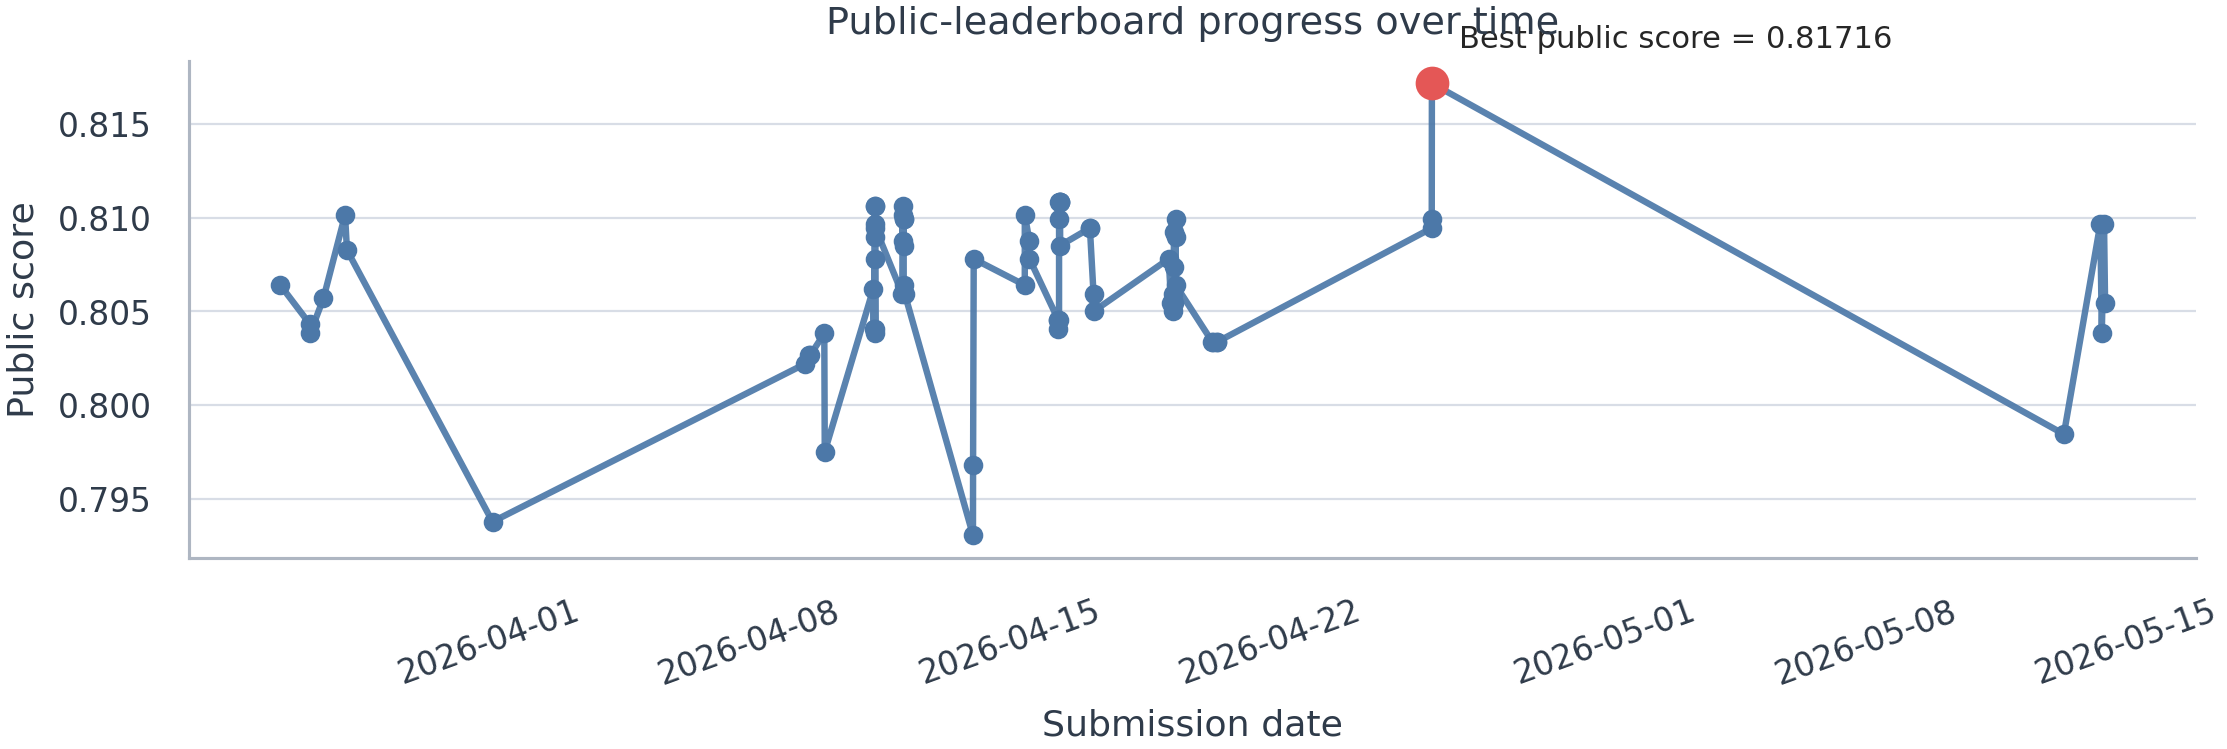
\includegraphics[width=\columnwidth]{submission_timeline.png}
\caption{Public leaderboard progress over time. The best visible submission remains the XGBoost branch submitted on April 26, 2026.}
\label{fig:timeline}
\end{figure}

\begin{figure}[!t]
\centering
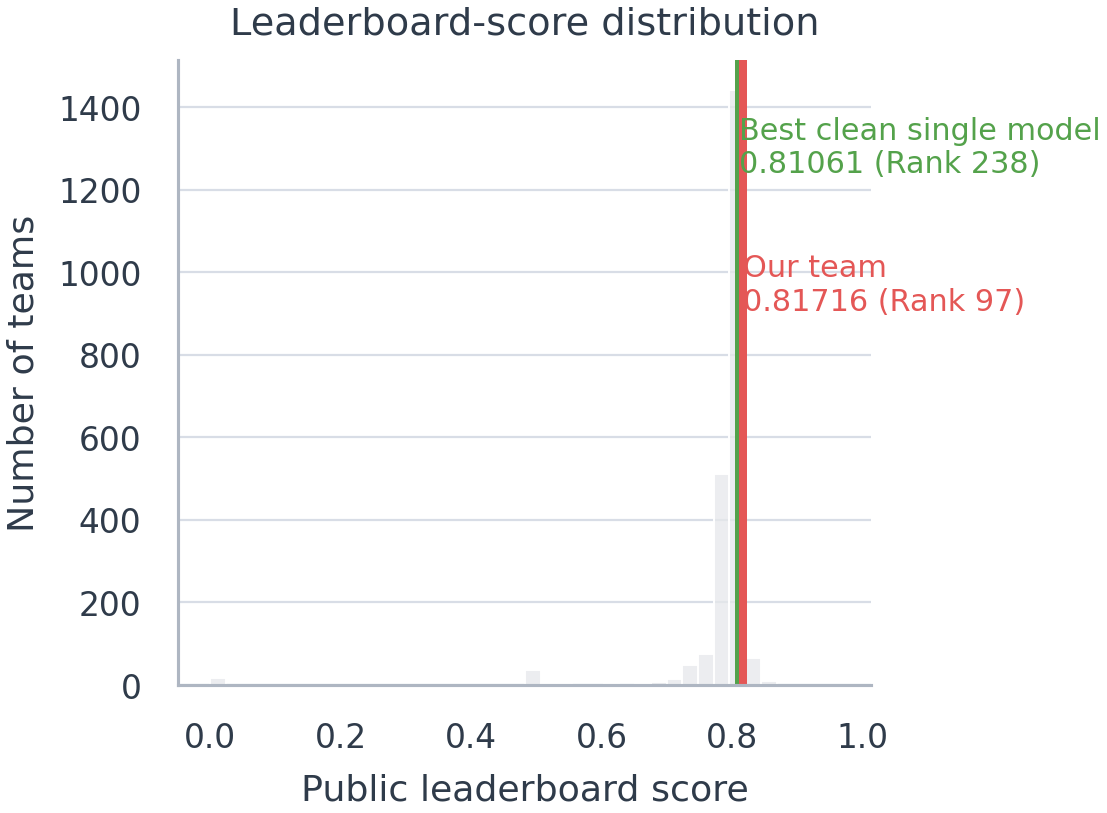
\includegraphics[width=\columnwidth]{leaderboard_context.png}
\caption{Leaderboard-score distribution in the public snapshot downloaded on May 17, 2026. The team result and the best clean single-model result are highlighted.}
\label{fig:leaderboard}
\end{figure}

\begin{figure*}[!t]
\centering
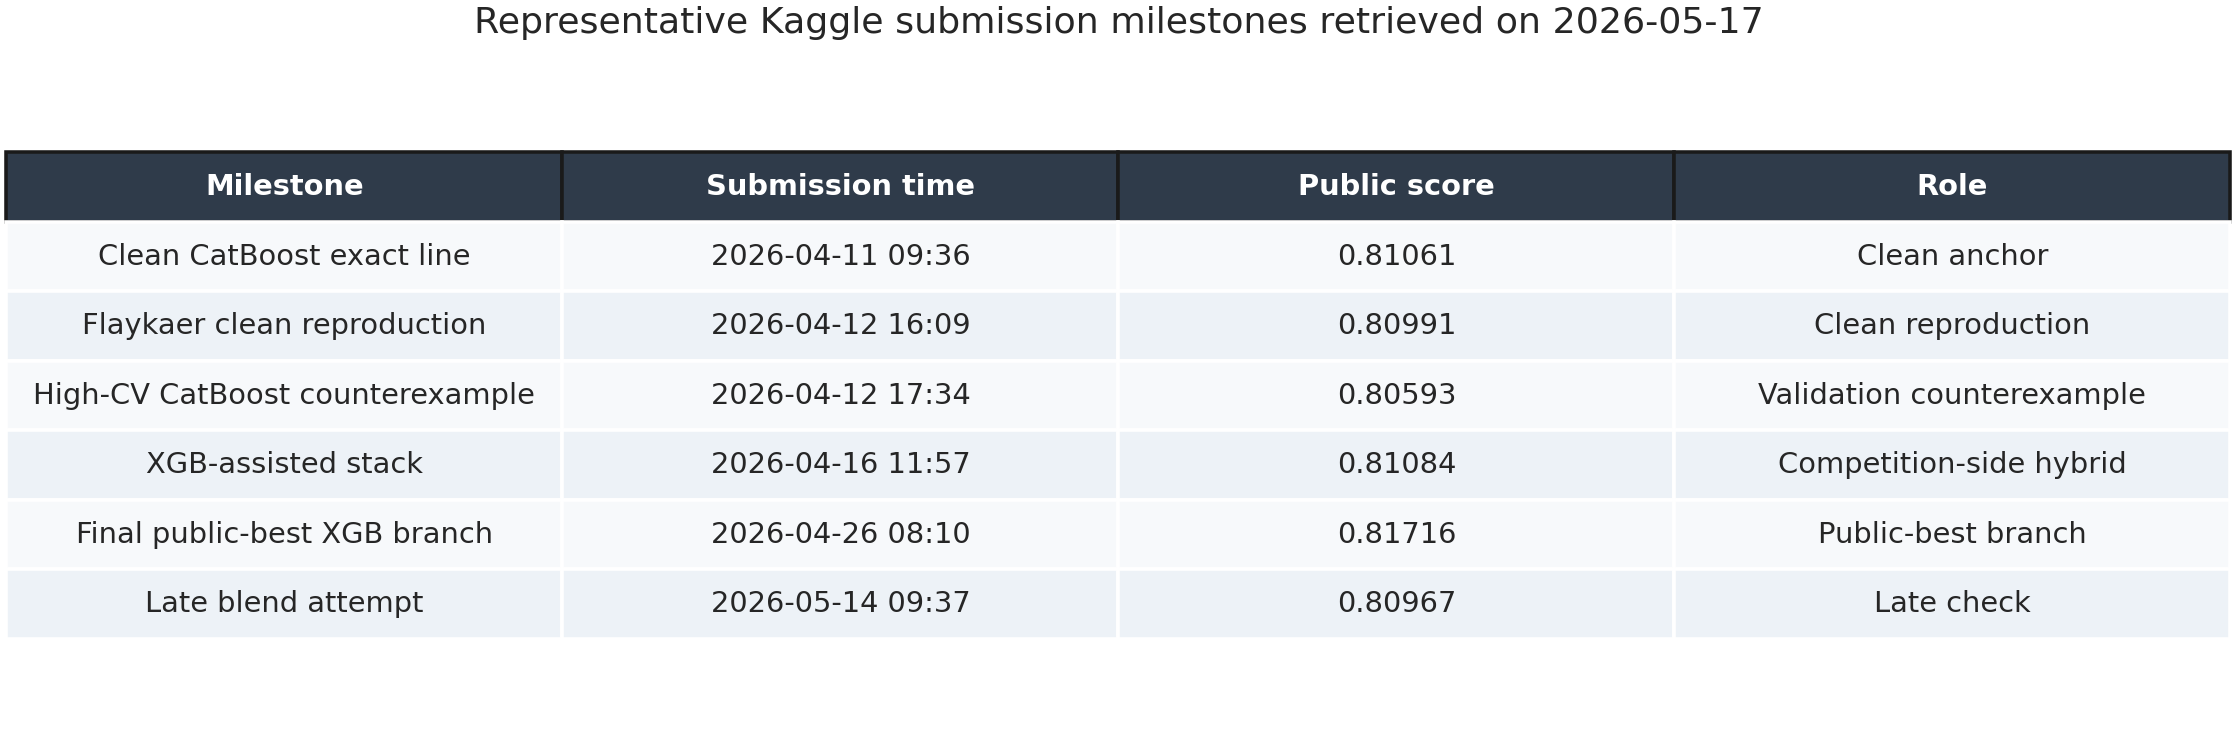
\includegraphics[width=0.96\textwidth]{submission_log_snapshot.png}
\caption{Representative Kaggle submission milestones retrieved on May 17, 2026. Semantic labels are used in place of raw file names; the best visible score is the final public-best XGBoost branch at 0.81716.}
\label{fig:submissionlog}
\end{figure*}

\section{Discussion}
Three lessons are worth emphasizing.

First, \emph{Spaceship Titanic} is not a good setting for uncritical leaderboard chasing if the goal is an academically strong report. Because the dataset is small and highly exposed, public-score changes can reflect split-specific behavior rather than reliable generalization. This concern is consistent with prior work on leaderboard reliability, which treats repeated public-score interaction as a genuine evaluation problem rather than a harmless convenience \cite{ladder}.

Second, the strongest clean single-model pipeline and the strongest public-scoring pipeline are not the same object. The CatBoost exact line is the best narrative anchor for a classroom report because it is transparent, stable, and easy to justify. The public-best XGBoost branch is the correct competition artifact because it demonstrably delivered the highest team score. Treating these two roles separately resolves the main tension in the project.

Third, the most valuable scientific contribution of the work is the validation framework itself. The repeated group-aware design, the split between search seeds and audit seeds, and the refusal to promote 0.000x gains without wider checking all made the project more trustworthy. On this dataset, that discipline is more important than any last 0.00x leaderboard fluctuation.

\section{Threats to Validity}
This project has three main validity threats.

First, the public leaderboard is only a partial view of the hidden Kaggle test set. Even a real public gain may not transfer perfectly to the private split. This is why the paper does not equate public-best score with universal model superiority.

Second, the competition-side XGBoost branch uses choices that are more acceptable in a competition than in a clean scientific benchmark, especially train-plus-test harmonization and manual encoded-feature pruning. We therefore describe it explicitly as a competition-side branch rather than as the main scientific conclusion.

Third, the whole study is still conducted inside one competition ecosystem. Even though our validation discipline is stronger than a naive single split, the conclusions remain about \emph{Spaceship Titanic} specifically and should be read as a careful case study in tabular competition methodology.

\section{Future Work and Conclusion}
If we were extending the project beyond the course deadline, the next priorities would not be another leaderboard-oriented adjustment. More meaningful directions would be nested group-aware hyperparameter tuning, fold-wise error analysis for group-consistency failures, probability calibration, and stability checks on feature-importance explanations. A more detailed probability-level analysis of the CatBoost--XGBoost disagreement regions would also strengthen the interpretability story.

In conclusion, the project achieved both of its goals, but through different model lines. On the competition side, the team reached 0.81716 and Rank 97/2240 in the public leaderboard snapshot dated May 17, 2026. On the methodological side, the report established a reproducible validation-first workflow, benchmarked five models, documented computational trade-offs, and showed that local validation and public leaderboard behavior can diverge sharply in both directions. For a getting-started Kaggle dataset such as \emph{Spaceship Titanic}, that final lesson is arguably the most valuable one: robust conclusions come from disciplined validation and careful ablation, not from equating a public leaderboard improvement with scientific truth.

\section{Code Availability and Contribution Statement}
\subsection{Code Availability}
The final IEEE paper, generated figures, tables, and supporting scripts are organized under the \texttt{final\_ieee\_paper} workspace folder. The copied data, notes, and benchmark tables used to regenerate the report are organized under the \texttt{paper\_support} folder in the same project root. A verified GitHub repository URL is not present anywhere in the shared workspace at the time of writing, so the final institutional submission should replace the placeholder below with the team's actual repository:

\begin{center}
\texttt{<insert-team-github-repository-url-here>}
\end{center}

\subsection{Contribution Statement}
The course requires a member-level contribution statement. The shared workspace does not contain a verified mapping from official student names to workstreams, so the final institutional submission should replace the placeholder text below with the team's confirmed allocation.

The workstreams that need explicit student mapping are:
\begin{enumerate}
\item EDA and feature engineering design
\item validation protocol design and benchmark implementation
\item competition-side XGBoost exploration and Kaggle submission management
\item final paper integration, figure generation, and presentation preparation
\end{enumerate}

\appendices
\section{Requirement Traceability}
Table~\ref{tab:requirement-map} maps the course report requirements to concrete evidence in this paper.

\begin{table*}[!t]
\caption{Traceability from course requirements to evidence in the final paper}
\label{tab:requirement-map}
\centering
\scriptsize
\begin{tabularx}{\textwidth}{>{\raggedright\arraybackslash}p{0.26\textwidth}X}
\toprule
Course requirement & Evidence in this paper \\
\midrule
Abstract & Abstract section on page 1 summarizes the task, methods, and final outcomes. \\
Introduction & Section I explains the competition setting and the distinction between leaderboard outcome and scientific claim. \\
Related work / existing techniques & Section II discusses boosting models, validation practice, and representative Kaggle guides. \\
Methodology & Section IV documents preprocessing, feature engineering, validation design, and the competition-side XGBoost branch. \\
Experimental study and results analysis & Section V contains the unified benchmark, CV-public alignment analysis, XGBoost branch reconstruction, and final ranking discussion. \\
Future work and conclusion & Section VIII provides both next steps and final conclusions. \\
References & The bibliography cites the competition page, model papers, Optuna, and representative Kaggle notebooks. \\
Contribution statement & Section IX contains the required contribution structure and the placeholder that should be replaced with verified student mapping. \\
Final Kaggle ranking & Section V-E and Figures~\ref{fig:timeline}--\ref{fig:leaderboard} report Rank 97/2240 with public score 0.81716 in the May 17, 2026 snapshot. \\
GitHub link of the code & Section IX-A contains the repository placeholder because no verified URL exists in the shared workspace. \\
Screenshot(s) of Kaggle submission log(s) & Figure~\ref{fig:submissionlog} provides a cleaned submission-log snapshot with representative milestones retrieved on May 17, 2026. \\
\bottomrule
\end{tabularx}
\end{table*}

\section{Milestone Submission Record}
Table~\ref{tab:milestone-record} records the milestone submissions that matter most to the final narrative.

This appendix is included for two practical reasons. First, the course requires evidence of the final Kaggle workflow rather than only the final score. Second, the main body of the paper repeatedly distinguishes between clean scientific anchors and competition-side artifacts; the milestone list makes that distinction concrete in submission-history terms.

\begin{table*}[!t]
\caption{Milestone submission record used in the final analysis}
\label{tab:milestone-record}
\centering
\scriptsize
\begin{tabularx}{\textwidth}{>{\raggedright\arraybackslash}p{0.12\textwidth}>{\raggedright\arraybackslash}p{0.20\textwidth}cp{0.16\textwidth}X}
\toprule
Date & Milestone label & Public score & Pipeline type & Why it matters \\
\midrule
2026-04-11 & Clean CatBoost exact line & 0.81061 & Clean single model & Best clean single-model anchor used for most of the report narrative. \\
2026-04-12 & Flaykaer clean reproduction & 0.80991 & Clean reproduction & Transparent group-aware CatBoost reproduction that remained interpretable but did not beat the clean anchor. \\
2026-04-12 & High-CV CatBoost counterexample & 0.80593 & High-CV clean candidate & Strong local-CV counterexample showing that public and local metrics can diverge sharply. \\
2026-04-16 & XGB-assisted stack & 0.81084 & Competition-side hybrid & Demonstrates that XGBoost became useful before the final public-best branch. \\
2026-04-26 & Final public-best XGB branch & 0.81716 & Competition-side compact branch & Highest public score in the team history and the endpoint of the XGBoost exploration path. \\
2026-05-14 & Late blend attempt & 0.80967 & Late ensemble check & Confirms that later submissions did not surpass the April 26, 2026 public best. \\
\bottomrule
\end{tabularx}
\end{table*}

Read together with Figure~\ref{fig:timeline}, this appendix clarifies the project chronology. The April 26, 2026 XGBoost branch remained the best visible public result through the final snapshot on May 17, 2026, while the cleaner CatBoost line remained the report's main scientific anchor. That dual interpretation is central to the paper and is therefore documented explicitly here.

\balance
\begin{thebibliography}{99}

\bibitem{kaggle}
Kaggle, ``Spaceship Titanic,'' online competition page. Available: \url{https://www.kaggle.com/competitions/spaceship-titanic/overview}

\bibitem{xgboost}
T. Chen and C. Guestrin, ``XGBoost: A scalable tree boosting system,'' in \emph{Proc. 22nd ACM SIGKDD Int. Conf. Knowledge Discovery and Data Mining}, 2016, pp. 785--794.

\bibitem{lightgbm}
G. Ke, Q. Meng, T. Finley, T. Wang, W. Chen, W. Ma, Q. Ye, and T.-Y. Liu, ``LightGBM: A highly efficient gradient boosting decision tree,'' in \emph{Advances in Neural Information Processing Systems}, 2017.

\bibitem{catboost}
L. Prokhorenkova, G. Gusev, A. Vorobev, A. V. Dorogush, and A. Gulin, ``CatBoost: unbiased boosting with categorical features,'' in \emph{Advances in Neural Information Processing Systems}, 2018.

\bibitem{rf}
L. Breiman, ``Random forests,'' \emph{Machine Learning}, vol. 45, no. 1, pp. 5--32, 2001.

\bibitem{sklearn}
F. Pedregosa \emph{et al.}, ``Scikit-learn: Machine learning in Python,'' \emph{Journal of Machine Learning Research}, vol. 12, pp. 2825--2830, 2011.

\bibitem{optuna}
T. Akiba, S. Sano, T. Yanase, T. Ohta, and M. Koyama, ``Optuna: A next-generation hyperparameter optimization framework,'' in \emph{Proc. 25th ACM SIGKDD Int. Conf. Knowledge Discovery and Data Mining}, 2019, pp. 2623--2631.

\bibitem{ladder}
A. Blum and M. Hardt, ``The Ladder: A reliable leaderboard for machine learning competitions,'' in \emph{Proc. 32nd Int. Conf. Machine Learning}, 2015, pp. 1006--1014.

\bibitem{cortinhas}
S. Cortinhas, ``Spaceship Titanic: A complete guide,'' Kaggle notebook, 2022. Available: \url{https://www.kaggle.com/code/samuelcortinhas/spaceship-titanic-a-complete-guide}

\bibitem{arunklenin}
Arunklenin, ``Space Titanic | EDA | Advanced Feature Engineering,'' Kaggle notebook, 2024. Available: \url{https://www.kaggle.com/code/arunklenin/space-titanic-eda-advanced-feature-engineering}

\end{thebibliography}

\end{document}
